\documentclass[times, utf8, diplomski]{fer}
\usepackage{booktabs}
\usepackage{float}
\usepackage{subcaption}
\usepackage[ruled, vlined]{algorithm2e}
\usepackage{amsmath}
\usepackage{listings}	
\usepackage{color}

\definecolor{backcolour}{rgb}{0.95,0.95,0.92}

\lstdefinestyle{mystyle}{
	backgroundcolor=\color{backcolour},
}

\lstset{style=mystyle}

\newcommand{\source}[1]{\vspace{-12pt} \caption*{\textbf{Source}: {#1}} }
\renewcommand{\labelitemi}{\textbullet}

\begin{document}

% TODO: Navedite broj rada.
\thesisnumber{000}

% TODO: Navedite naslov rada.
\title{Brojanje ljudi u sceni}

% TODO: Navedite vaše ime i prezime.
\author{Luka Novak}

\maketitle

% Ispis stranice s napomenom o umetanju izvornika rada. Uklonite naredbu \izvornik ako želite izbaciti tu stranicu.
\izvornik

% Dodavanje zahvale ili prazne stranice. Ako ne želite dodati zahvalu, naredbu ostavite radi prazne stranice.
\zahvala{}

\tableofcontents

\chapter{Uvod}
Kada se govori o biologiji i medicini, dvije grane koje se bave proučavanjem života i načina funkcioniranja živih bića, svi se slažu da su izuzetno puno napredovale sa razvojem tehnologije. Ljudi razvijaju sve složenije i sve preciznije alate, strojeve i programe za proučavanje svih sustava u tijelu, od stanice do skupa organa koji rade zajedno, kao jedan, te skupa čine savršeno ugođeni sustav. No u jednom području tih znanosti ne napreduje se tom brzinom kao u ostalim područjima. O tom području i sustavu organa nezna niti približno mnogo kao o ostalim organima i sustavima u tijelu. Znanstvenici govore da je to najsloženiji sustav, najjače super-računalo na svijetu. Centar tog sustava je mozak, organ koji može probaviti nevjerojatnu količinu informacija u stvarnom vremenu sa gotovo savršenom preciznosti. \par

Od početka "modernog doba čovječanstva", javlja se ideja umjetne inteligencije. Znanstvenici iz područja tehničkih znanosti i računarstva teže razvijanju nečeg takvog i prirodno se nameće ljudski mozak kao ideal, razina inteligencije koju se želi dostići. Pretpostavlja se da je najveći dio mozga, oko 2/3, posvećen vidu \citep{vision_percentage}. Iz tog razloga, veliki dio proučavanja i razvoja moderne umjetne inteligencije fokusirano je na vid. U nastavku rada dan je pregled najvažnijih algoritama i arhitektura mreža.

\chapter{Računalni vid}
\section{Računalni vid}
Računalni vid je veliko područje računarske znanosti koje se bavi algoritmima i metodama vezanim za obradu slike. Kao što je navedeno u uvodu, vid je osjetilo preko kojega ljudi primaju najviše informacija, više nego preko bilo kojeg drugog osjetila. Da bi bilo moguće napraviti stroj ili program koji vidi kao mi, prvo je potrebno shvatiti kako ljudi vide i kako obrađuju informacije primljene preko očiju. Samo shvaćanje kako funkcionira ljudski vid je izuzetno težak zadatak. Danas donekle razumijemo taj proces, no ima još puno stvari koje su ostale neodgovorene. Recimo, istraživanja pokazuju da ljudi mogu prepoznati što je na slici za samo 13 milisekundi\citep{RSVP13ms}. Ljudi i dalje ne znaju kako mozak to radi. Postoje nagađanja, no ništa nije dokazano i upitno je hoće li ikada ti koncepti biti do kraja shvaćeni i objašnjeni. Zbog složenosti ovog problema, nemoguće je naći riješenje klasičnim pristupom i napisati program eksplicitno. Zato se u ovakvim problemima pribjegava umjetnoj inteligenciji.
Postoji nekoliko dijelova cijelog sustava vida koji ljudima omogućavaju vid:
\begin{itemize}
\item{\textbf{Vidjeti}} - dati računalu vid znači dati mu oči. U tom području znanost je dosta napredovala tako da danas postoje kamere sa većom rezolucijom od ljudskog oka. Ovaj dio vida odvija se, naravno, u samom oku.
\item{\textbf{Prepoznati}} - moći prepoznati različite objekte, maknuti šum sa slike itd. Ukratko, vidjeti što se na slici nalazi. Ovaj aspekt vida odvija se unutar oka i na putu do mozga gdje mozak na kraju posloži sve te informacije u smislenu sliku.
\item{\textbf{Razumijeti}} - shvatiti što se na slici nalazi, shvatiti odnose među objektima, propoznati različite predmete iz različitih kuteva... Ljudski mozak sposoban je prepoznati jabuku bila ona crvena, žuta ili zelena. Sposoban je prepoznati jabuku i ako je napola pojedena. Sposoban je prepoznati jabuku neovisno o njenoj orjentaciji, neovisno o tome miruje li ili se kreće. Ovaj dio vida odvija se potpuno u mozgu. Ovdje je trenutno dosegnuta granica računalnog vida i umjetne inteligencije. No, to ne znači da je nemoguće ići dalje, nego samo da je znanost savladala dosadašnje probleme i trenutno se bavi ovim dok ne nađe riješenje. 
\end{itemize}

\section{Kategorije računalnog vida}
Računalni vid podjeljen je u nekoliko kategorija:
\begin{enumerate}
\item \textbf{Klasifikacija i Lokalizacija.} Ovo područje računalnog vida bavi se prepoznavanjem objekata na slici. To znači da algoritam odlučuje kojem razredu (\textit{engl.} class) pripada cijela slika. Pretpostavljajući navedeno, lokalizacija je proces pronalaženja pozicije objekta na slici. Rezultat procesa lokalizacije obično je crtanje okvira (\textit{engl.} bounding box) oko objekta na slici. Pobjednici natjecanja "Large Scale Visual Recognition Challenge 2017 (ILSVRC2017)" u kategoriji klasifikacije pobijedili su sa rezultatom od 2.251\% pogreške, dok su pobjednici u kategoriji lokalizacije postigli rezultat sa greškom od 6.226\%. Sa slike \ref{img:ILSVRC} vidi se da su se razultati u odnosu na 2016. godinu popravili za 0.8\% u kategoriji klasifikacije te 1.5\% u kategoriji lokalizacije .
\begin{figure}[htb]
\centering
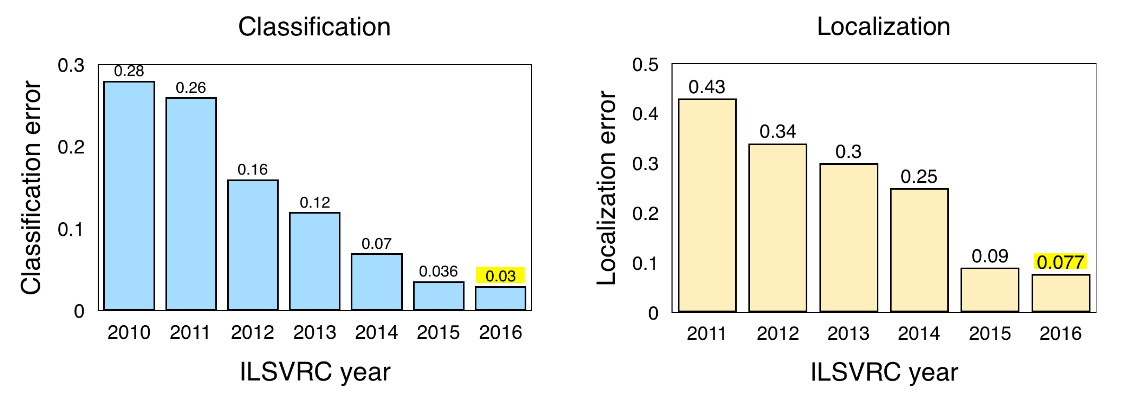
\includegraphics[width=\linewidth]{img/ILSVRC.png}
\caption{Rezultati natjecanja ILSVRC tijekom godina \citep{ILSVRC}}
\label{img:ILSVRC}
\end{figure}

\item \textbf{Detekcija.} Pod pojmom detekcija podrazumijeva se pronalaženje objekata na slici, odnosno, određivanje prisutnosti objekata na slici. Proces detekcije objekata je malo složeniji od kalsifikaije/lokalizacije objekata zbog toga što se ovdje mora provesti više klasifikacija i lokalizacija na jednoj slici te objekti mogu biti iz više domena. Pri klasifikaciji projeravamo pripada li objekt nekom razredu objekata i dobijamo binarni odgovor (\textit{pripada} ili \textit{ne pripada} dani objekt danom razredu), dok je pri detekciji potrebno provesti taj postupak za sve moguće razrede objekata.
\begin{figure}[htb]
\centering
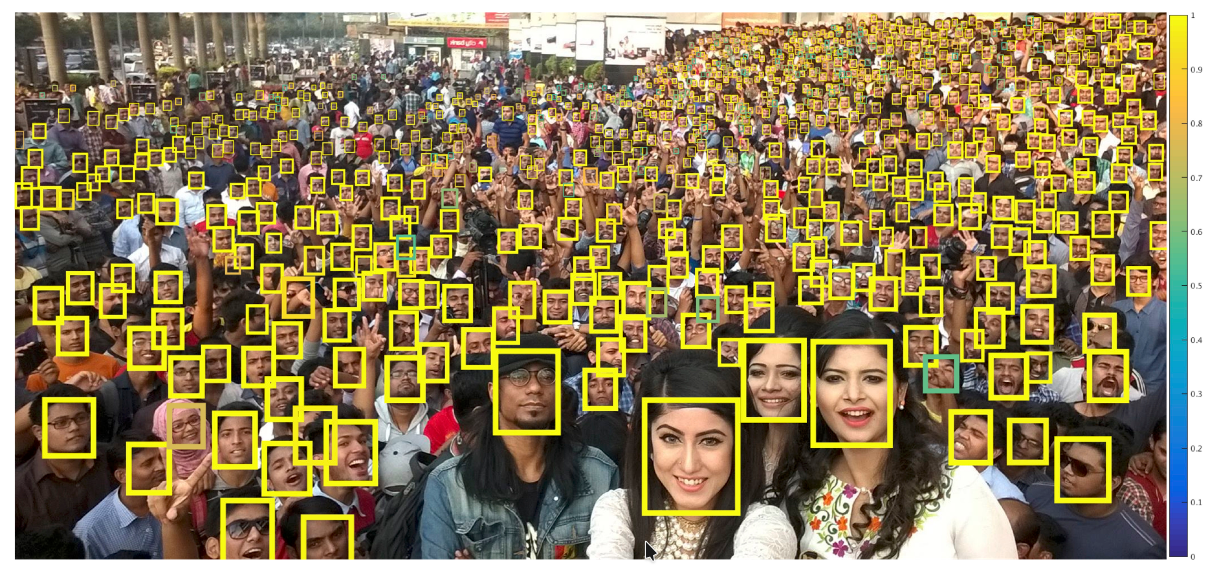
\includegraphics[width=\linewidth]{img/FindingTinyFaces.png}
\caption{Rezultati algoritma za detekciju lica iz rada \citep{TinyFaceDetector}}
\label{img:findingTinyFaces}
\end{figure}

\item \textbf{Praćenje.} Ovaj pojam odnosi se na praćenje određenog objekta ili više njih u sceni. Ova kategorija se, logično, primjenjuje samo u području videa i izuzetno je bitna za sustave koji riješavaju zadatke poput autonomne vožnje.

\item \textbf{Segmentacija.} Pojam segmentacije odnosi se na proces grupiranja piksela u skupine s kojima se kasnije može raditi niz drugih procesa, npr. klasifikacija itd. 

\begin{figure}[htb]
	\centering
	\begin{subfigure}[b]{0.4\linewidth}
		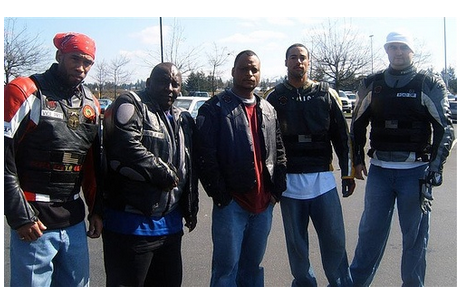
\includegraphics[width=\linewidth]{img/OriginalImage.png}
		\caption{Originalna slika}
	\end{subfigure}
	\begin{subfigure}[b]{0.4\linewidth}
		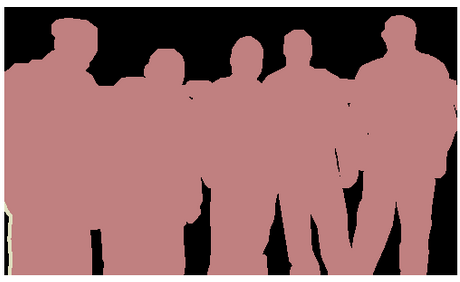
\includegraphics[width=\linewidth]{img/ImageSegmentation.png}
		\caption{Segmentirana slika}
	\end{subfigure}
	\caption{Segmentacija slike (Pascal VOC2007)}
	\label{img:segmentation}
\end{figure}

Nadalje, semantička segmenatacija, kako i samo ime govori, pokušava odrediti semantičku ulogu svakog piksela u slici. Dakle, možemo reći da pokušava klasificirati svaki piksel u njegovu semantičku cjelinu. 

\begin{figure}[htb]
\centering
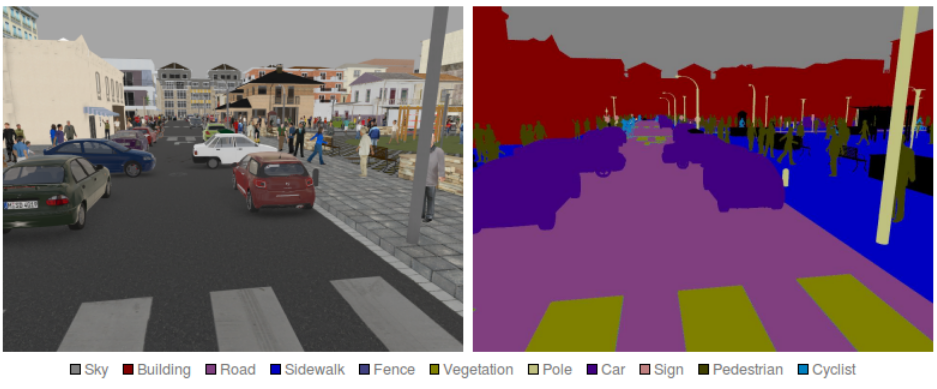
\includegraphics[width=\linewidth]{img/SemanticSegmentation.png}
\caption{Semantička segmentacija slike (SYNTHIA skup podataka)}
\label{img:semanticSegmentation}
\end{figure}

Instancijska segmentacija (\textit{engl.} Instance segmentation) ide i korak dalje. Ona pokušava segmentirati različite objekte istog razreda objekata. Primjerice, ako se na slici nalaze tri mobitela, svaki mobitelj bit će označen drugom bojom.

\begin{figure}[htb]
	\centering
	\begin{subfigure}[b]{0.4\linewidth}
		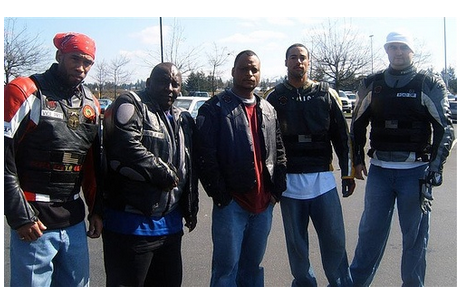
\includegraphics[width=\linewidth]{img/OriginalImage.png}
		\caption{Originalna slika}
	\end{subfigure}
	\begin{subfigure}[b]{0.4\linewidth}
		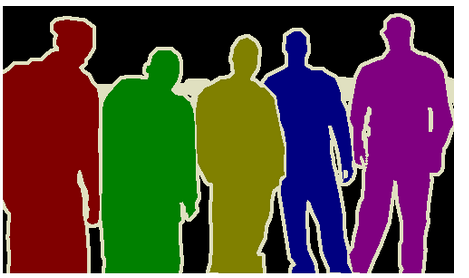
\includegraphics[width=\linewidth]{img/InstanceSegmentation.png}
		\caption{Instancijski segmentirana slika}
	\end{subfigure}
	\caption{Instancijska segmentacija slike, (Pascal VOC2007)}
	\label{img:instanceSegmentation}
\end{figure}

\bigskip
\item Ostale, manje zastupjene, kategorije računalnog vida : Super-resolution, Style Transfer, Colourisation 

\begin{figure}[htp]
	\centering
	\begin{subfigure}[b]{0.4\linewidth}
		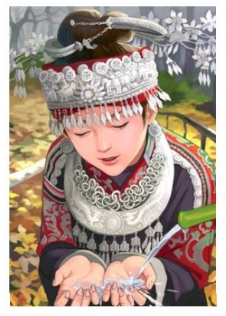
\includegraphics[width=\linewidth]{img/OriginalSRGAN.png}
		\caption{Originalna slika}
	\end{subfigure}
	\begin{subfigure}[b]{0.4\linewidth}
		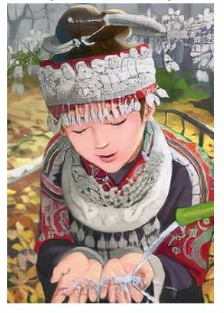
\includegraphics[width=\linewidth]{img/SRGAN.png}
		\caption{SRGAN}
	\end{subfigure}
	\caption{Slika poboljšana metodom Super-resolution GAN (Christian Ledig et al., 2016)}
	\label{img:SRGAN}
\end{figure}

\begin{figure}[htp]
	\centering
	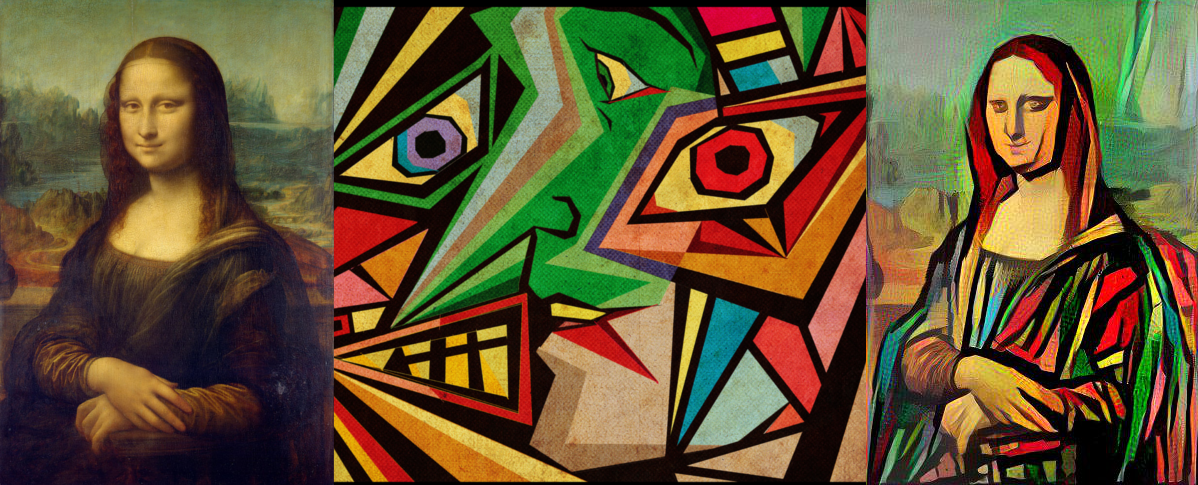
\includegraphics[width=\linewidth]{img/StyleTransfer.png}
	\caption{Prva slika prikazuje originalnu \textit{Mona Lisu}, druga slika prikazuje sliku naslikanu u stilu kubizma/ekspresionizma, treća slika prikazuje stil druge slike prenesen na prvu sliku}
	\label{img:styleTransfer}
\end{figure}

\begin{figure}[H]
	\centering
	\begin{subfigure}[b]{0.4\linewidth}
		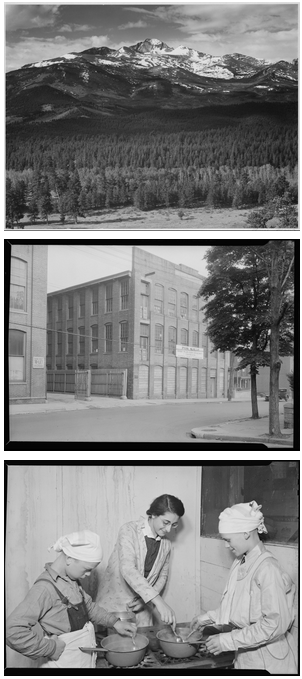
\includegraphics[width=\linewidth]{img/ColourisationOriginal.png}
		\caption{Originalna slika}
	\end{subfigure}
	\begin{subfigure}[b]{0.4\linewidth}
		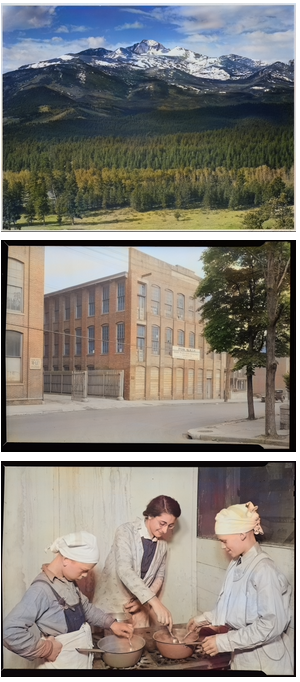
\includegraphics[width=\linewidth]{img/Colourisation.png}
		\caption{Colourisation}
	\end{subfigure}
	\caption{Slika poboljšana metodom colourisation}
	\label{img:colourisation}
\end{figure}

\end{enumerate}

U okviru ovoga rada pažnja je stavljena isključivo na \textbf{detekciju objekata}.

\chapter{Detekcija objekata prije konvolucijskih modela}
Povijest prepoznavanja (detekcije) objekata seže puno dalje od konvolucijskih neuronskih mreža. Prvi sustavi detekcije objekata problemu su prilazili geometrijski. Neki od takvih pristupa bili su:

\begin{itemize}
\item \textbf{poravnanje} gdje se pokušavalo pronaći takvu transformaciju slike koja bi minimizirala pogrešku:
\[\sum_{i} residual(T(x_i), x_i')\]

Ovaj period trajao je od ranih 60ih do početka 90ih godina prošlog stoljeća. Uglavnom se pokušavalo riješiti problem detekcije razlamanjem objekata na slici u manje komponente (\textit{engl. Block world}, L. G. Roberts Machine Perception of Three Dimensional Solids, 1963.).
\item \textbf{modeli temeljeni na izgledu} (\textit{engl. appearance - based models}) su modeli temeljeni na svojstvenim vrijednostima (Eigenfaces for Recognition, Turk and Pentland, 1991.) te histogramima boja (Swain and Ballard, IJCV 1991.)
\item \textbf{klizeći prozor} pristup koji se donekle i danas primjenjuje. Ovaj pristup smatra se početkom "modernog doba" računalnog vida, iako se klizeći prozor koristi u najjednostavnijijm mogućim oblicima. Ovaj period počinje ranih 90ih godina, a predvode ih Turk and Pentland svojim radom "Eigenfaces for Recognition" izdanim 1991. godine, a vrhunac se potiže 2001. godine objavljivanjem algoritma koji su razvili Viola i Jones.
\item \textbf{lokalne značajke} (\textit{engl. local features}) gdje su oblici predmeta koje je potrebno detektirati djelomično poznati (D. Lowe, 2004.). U tom periodu Google razvija i prvi pretraživač slika. 
\item \textbf{parts-and-shape modeli} koji koriste kombinaciju više vrsta značajki: ponovo razlamaju objekte na dijelove, relativne odnose između tih dijelova te samu prisutnost dijelova objekta (Weber, Welling and Perona, 2000.).
\item \textbf{bags-of-features modeli} uvode prepoznavanje tekstura. Klasični bag-of-features modeli imaju standardizirane korake (\textit{engl. pipeline}): 
\begin{enumerate}
\item Feature extraction
\item Learn "visual vocabulary"
\item Quantize features using visual vocabulary
\item Represent images by frequencies of “visual words”
\end{enumerate}
\end{itemize}
\section{Viola-Jones algoritam}

Prije velikog razvoja konvolucijskih neuronskih mreža, Paul Viola i Michael Jones su 2001. godine u svom radu \citep{ViolaJones} objavili svoj algoritam koji je tada bio prvi algoritam koji je omogućavao detekciju lica u stvarnom vremenu. Iako se može trenirati i na drugim domenama, algoritam je najpoznatiji po detekciji lica pa će na toj domeni ovdje biti i opisan.

Naravno, algoritam treba puno pozitivnih (slike lica) i negativnih primjera (slike bez lica). Iz tih slika potrebno je izvući značajke prema kojima će kasnije biti moguće odrediti (detektirati) lice. Za ekstraciju značajki koriste se Haarove značajke.

\begin{figure}[htb]
	\centering
	\begin{subfigure}[b]{0.4\linewidth}
		
\includegraphics[width=\linewidth]{img/EdgeFeatures.png}
		\caption{Značajke rubova}
		\label{img:haar-features1}
	\end{subfigure}
	\begin{subfigure}[b]{0.4\linewidth}
		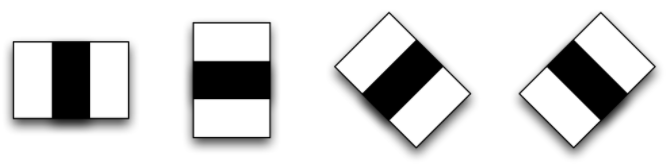
\includegraphics[width=\linewidth]{img/LineFeatures.png}
		\caption{Linijske značajke}
		\label{img:haar-features2}
	\end{subfigure}
	\begin{subfigure}[b]{0.4\linewidth}
		
\includegraphics[width=\linewidth]{img/DiagonalFeatures.png}
		\caption{Dijagonalne značajke}
		\label{img:haar-features3}
	\end{subfigure}
	\begin{subfigure}[b]{0.4\linewidth}
		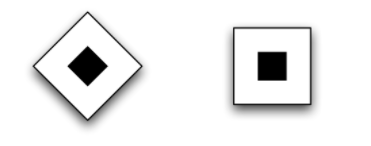
\includegraphics[width=\linewidth]{img/CenterSorround.png}
		\caption{Radijalne značajke}
		\label{img:haar-features4}
	\end{subfigure}
	\caption{Haarove značajke}
	\label{img:haar-features}
\end{figure}

Haarove značajke računaju se na temelju razlike u intenzitetu piksela. Primjerice, ako su vrijednosti piksela u rasponu od 0 (bijeli piksel) do 1 (crni piksel), svi pikseli koji imaju vrijednost veću do 0.5 smatraju se tamnim, a svi pikseli koji imaju vrijednost manju od 0.5 smatraju se svijetlima. Na slici \ref{img:haar-features} prikazane su 4 kategorije Haarovih značajki. Dakle, kako bi bilo moguće odrediti gdje se na slici nalazi (i ako se nalazi) neka od značajki, slika se dijeli na manja područja te se na svakom od tih područja traže Haarove značajke. Naravno, značajke se skaliraju i rotiraju kako bi se pronašli svi dijelovi slike koji zadovoljavaju uvjete značajki. Zatim se odredi gledano područje, kao što to prikazuje slika \ref{img:haar-calc}, te se računaju vrijednosti za Haarove značajke po formuli:
\[
\Delta = dark - white = \frac{1}{n}\sum_{}^{n}I_{dark}(x) - \frac{1}{n}\sum_{}^{n}I_{light}(x)
\]

\begin{figure}[htb]
	\centering
	\begin{subfigure}[b]{0.4\linewidth}
		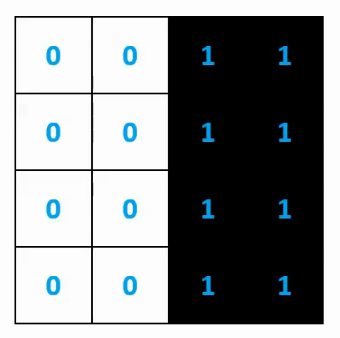
\includegraphics[width=\linewidth]{img/IdealHaarFeatures.png}
		\caption{Idealne vrijednosti piksela}
		\label{img:haar-ideal-features}
	\end{subfigure}
	\begin{subfigure}[b]{0.4\linewidth}
		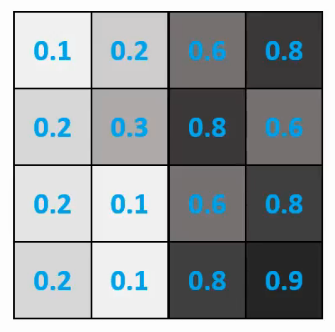
\includegraphics[width=\linewidth]{img/RealHaarFeatures.png}
		\caption{Stvarne vrijednosti piksela}
		\label{img:haar-real-features}
	\end{subfigure}
	\caption{Izračun za linijske Haarove značajke}
	\label{img:haar-calc}
\end{figure}


Slika \ref{img:haar-features1} prikazuje Haarove značajke rubova. Neke od primjena tih značajki su detekcija obrva, gornje/donje usne i zubi. Slika \ref{img:haar-features2} prikazuje linijske Haarove značajke koje služe za detekciju nosa, usta, očiju itd. Nadalje, slika \ref{img:haar-features3} prikazuje dijagonalne Haarove značajke koje se koriste u detekciji složenijih karakteristika. Recimo, ako se lice na slici smije, rubovi usana se uvuku u obraze te su tada slabije osvjetljeni. Tako zajedno sa okom na istoj strani lica tvore tamnije zone, dok obraz i nos čine svijetlija područja. Zadnja skupina Haarovih značajki su radijalne Haarove značajke koje prikazuje slika \ref{img:haar-features4}. Te se značajke koriste u detekciji zjenica, rubova usana i sl. Dakle, Haarove značajke mogu se shvatiti kao preteča konvolucijskih jezgri. Slika \ref{img:haar-image} prikazuje neke od haarovih značajki detektiranih na slici.

\begin{figure}[htb]
	\centering
	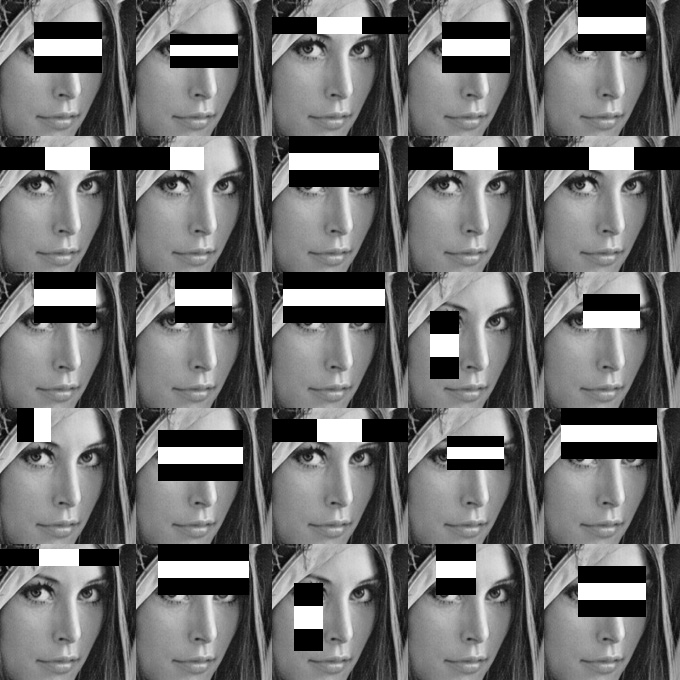
\includegraphics[width=12cm]{img/Haar3.jpg}
	\caption{Neke od Haarovih značajki pronađenih na slici}
	\label{img:haar-image}
\end{figure}

Ovaj proces je dosta spor i neefikasan jer se na ovakav način dođe do više od 160000 različitih značajki. Očito je da, ovisno o domeni, neke od značajki odgovaraju više od drugih, no javlja se pitanje kako odabrati najbolje značajke? Odgovor na ovo pitanje je Adaboost algoritam. Adaboost (skraćeno od \textit{engl. Adaptive Boosting}) je algoritam osmišljen 2003. godine koji kombinira izlaze iz ostalih, "slabijih" kalsifikatora, te njihovom težinskom sumom dolazi do optimuma algoritma. Adaboost zapravo uči i optimizira težine za svaki od klasifikatora.

\begin{figure}[htb]
	\centering
	
\includegraphics[width=\linewidth]{img/Viola-Jones.png}
	\caption{Viola-Jones algoritam}
	\label{img:viola-jones}
\end{figure}

Autori su došli do zaključka da je čak sa samo 200 značajki moguće postići točnost pronalaženja lica od 95\%. Konačne postavke algoritma iz rada \citep{ViolaJones} sadržavale su oko 6000 značajki. Kako bi optmimizirali ovaj složeni proces i izbjegli primjenu svih 6000 značajki na svaku sliku, Viola i Jones odlučili su napraviti strukturu kaskada značajki u kojoj svaka iduća razina ima sve složenije Haarove značajke. Kao što je označeno na slici \ref{img:haar-cascades}, svaka razina ima mogućnost odbaciti sliku ukoliko ne nađe značajke svoje razine na slici. Tako se dijelovi slike koji ne prikazuju lice odbacuju te se oslobađaju računalni resursi za procesiranje slika na kojima se nalazi lice. Autori navode da je prosjek značajki evaluiranih po slici oko 10.

\begin{figure}[htb]
	\centering
	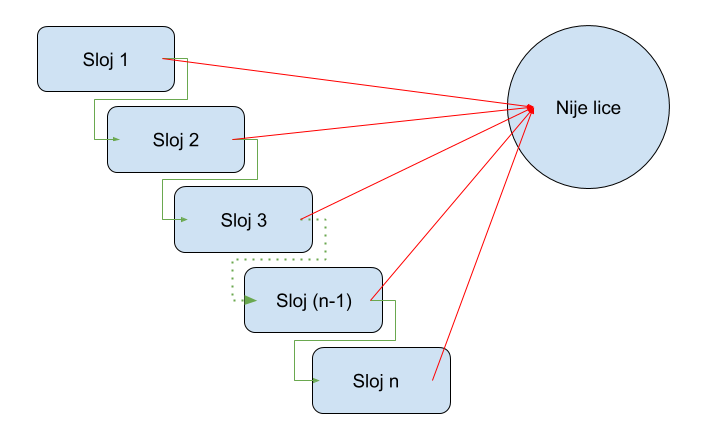
\includegraphics[width=\linewidth]{img/HaarCascades.png}
	\caption{Kaskada Haarovih značajki}
	\label{img:haar-cascades}
\end{figure}

\begin{figure}[htb]
	\centering
	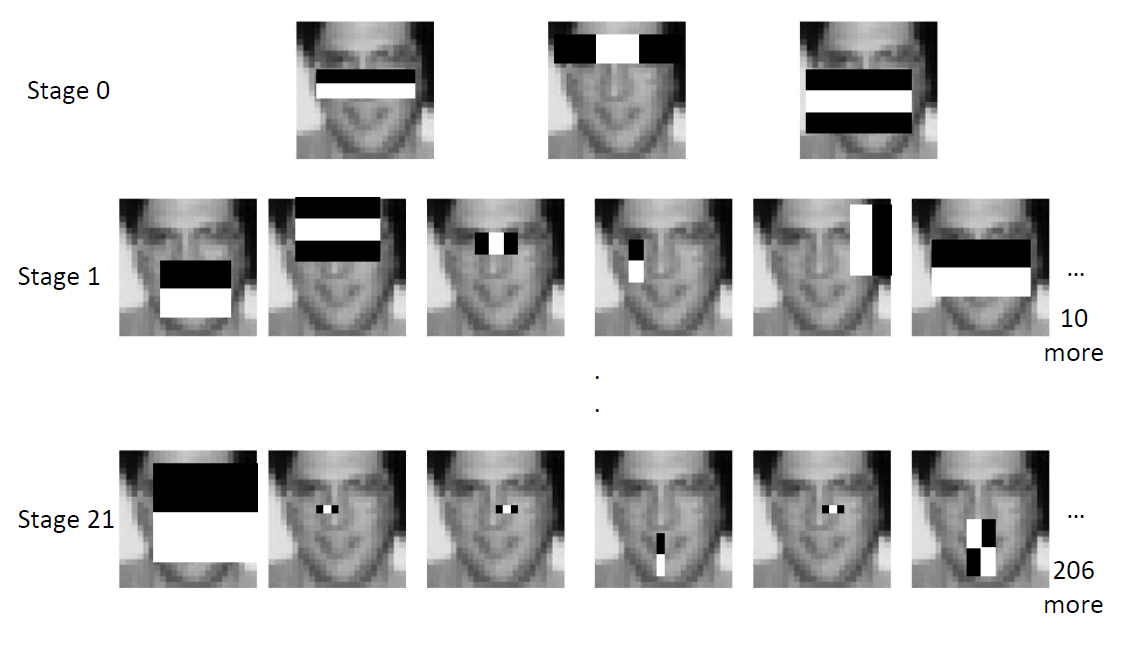
\includegraphics[width=\linewidth]{img/haar2.jpg}
	\caption{Dijelovi Haarovih značajki pronađeni na različitim razinama kaskada}
	\label{img:haar-cascade-layers}
\end{figure}

Rezultati ovih slabijih klasifikatora kombiniraju se u konačni klasifikator koji odlučuje nalazi li se lice na slici. 

Viola-Jones algoritam je svojedobno bio vrlo popularan algoritam jer nudi vrlo pouzdane rezultate, obradu u stvarnom vremenu i invarijantnost na skaliranje. No, isto tako, ima i nekoliko nedostataka kao što su netolerantnost na rotaciju, osjetljivost na osvjetljenje objekata na slici i sl. Činjenica da se još i danas koristi govori dovoljno o kvaliteti i važnosti ovog algoritma.


\chapter{Detekcija objekata konvolucijskim modelima}
\section{Neuronske mreže}

\subsection{Neuron}

Neuronske mreže nastale su kao rezultat pokušaja reprodukcije rada ljudskog mozga.

Osnovna gradivna jedinica ljudskog mozga jest neuron. Ljudski mozak sastavljen je od oko $10^11$ neurona kojih ima više od 100 vrsta i koji su shodno svojoj funkciji raspoređeni prema točno definiranom 
rasporedu. Svaki je neuron u prosjeku povezan s $10^4$ drugih neurona. Četiri su osnovna dijela neurona: tijelo stanice (soma), skup dendrita (ogranaka), aksona (dugačke cijevčice koje prenose električke poruke) i niza završnih članaka 

\begin{figure}[htb]
\centering
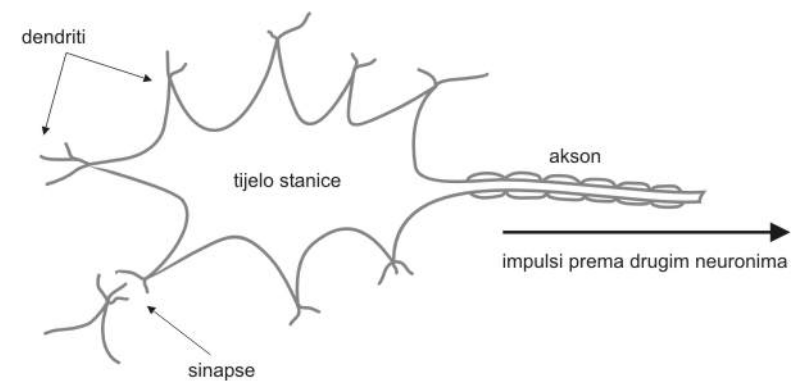
\includegraphics[width=8cm]{img/Neuron.png}
\caption{Građa neurona}
\label{img:human-neuron}
\end{figure}

Tijelo stanice sadrži informaciju predstavljenu električkim potencijalom između unutrašnjeg i vanjskog dijela stanice (oko –70 mV u neutralnom stanju). Na sinapsama, spojnom sredstvu dvaju neurona kojim su pokriveni dendriti, primaju se informacije od drugih neurona u vidu post-sinaptičkog potencijala koji utječe na potencijal stanice povećavajući (hiperpolarizacija) ili smanjivajući ga (depolarizacija). U tijelu stanice sumiraju se post-sinaptički potencijali tisuća susjednih neurona, u ovisnosti o vremenu dolaska ulaznih informacija. Ako ukupni napon pređe određeni prag, neuron "pali" i generira tzv. akcijski potencijal u trajanju od 1 ms. Kada se informacija akcijskim potencijalom prenese do završnih članaka, onda oni, ovisno o veličini potenijala, proizvode i otpuštaju kemikalije, tzv. neurotransmitere. To zatim ponovno inicira niz opisanih događaja u daljnjim neuronima. Propagacija impulsa očigledno je jednosmjerna. 

Funkcionalnost biološkog neurona imitira McCulloch-Pitts model umjetnog neurona, tzv. \textit{Threshold Logic Unit} (TLU). Model koristi slijedeću analogiju: signali su opisani numeričkim iznosom i na ulazu u neuron množe se težinskim faktorom koji opisuje jakost sinapse; signali pomnoženi težinskim faktorima zatim se sumiraju analogno sumiranju potencijala u tijelu stanice; ako je dobiveni iznos iznad definirana praga, neuron daje izlazni signal. 

U općenitom slučaju, umjetni neuron umjesto funkcije praga može imati i neku drugu funkciju, tzv. aktivacijsku funkciju (transfer funkcija, prijenosna funkcija). Općeniti model umjetnog neurona nalazi se na slici \ref{img:artificial-neuron}. U nastavku ćemo za pojam umjetni neuron ravnopravno koristiti i istovjetne pojmove: čvor ili jedinica. 

\begin{figure}[htb]
\centering
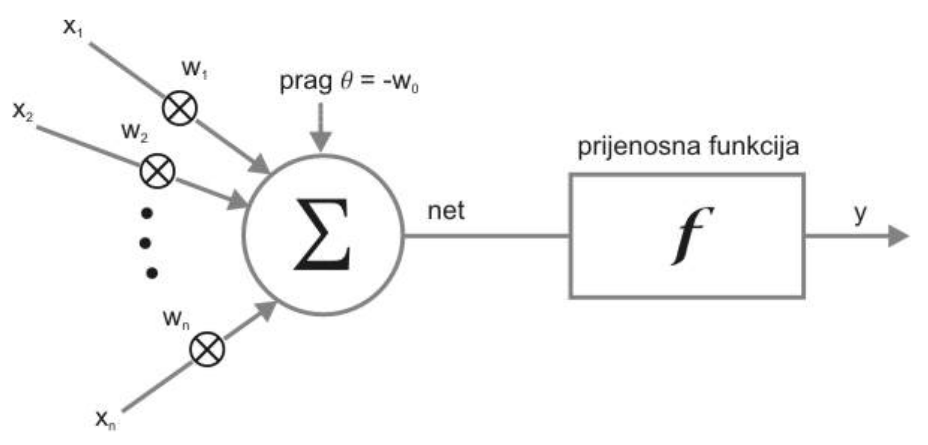
\includegraphics[width=8cm]{img/ArtificialNeuron.png}
\caption{Umjetni neuron}
\label{img:artificial-neuron}
\end{figure}

Ulazne signale (njih ukupno $n$) označavamo sa $x_1, x_2, x_3, ... , x_n$, a pripadajuće težine označavamo sa $\omega_1, \omega_2, \omega_3,..., \omega_n$.
Ulazni signali općenito su realni brojevi u intervalu $[-1,1]$, $[0,1]$ ili samo elementi iz $\{0,1\}$, kada govorimo o Booleovom ulazu. Težinska suma $net$ dana je formulom \ref{eq:weighted-sum}. Zbog kompaktnosti se često dogovorno uzima da je vrijednost praga $\theta = --\omega_0$ te se dodaje ulazni parametar $x_0$ s fiksiranom vrijednošću 1, te tada \ref{eq:weighted-sum} izgleda:

\begin{equation}
net = \omega_1 x_1 + \omega_2 x_2 + ... + \omega_n x_n - \theta
\label{eq:weighted-sum}
\end{equation}

\begin{equation}
net = \omega_0 x_0 + \omega_1 x_1 + \omega_2 x_2 + ... + \omega_n x_n = \sum_{i=0}^{n} \omega_i x_i
\label{eq:weighted-sum_2}
\end{equation}

Izlaz $y$ je rezultat aktivacijske funkcije te ga zapisujemo:

\begin{equation}
y = f(\sum_{i=0}^{n} \omega_i x_i) = f(net)
\label{eq:activation-function}
\end{equation}


\subsection{Svojstva umjetne neuronske mreže}

Umjetna neuronska mreža (\textit{engl.} Artificial Neural Network, ANN) u širem je smislu riječi umjetna replika ljudskog mozga kojom se nastoji simulirati postupak učenja. Nešto stroža definicija bila bi skup međusobno povezanih jednostavnih procesnih elemenata, \textit{jedinica} ili \textit{čvorova}, čija se funkcionalnost temelji na biološkom neuronu. Pri tome je obradbena moć mreže pohranjena u snazi veza između pojedinih neurona tj. težinama do kojih se dolazi postupkom prilagodbe odnosno učenjem iz skupa podataka za učenje. Neuronska mreža obrađuje podatke distribuiranim paralelnim radom svojih čvorova.

To je paradigma kojom su implementirani pojednostavljeni modeli što sačinjavaju biološku neuronsku mrežu. Ova je analogija vrlo poopćena jer, naravno, postoje još mnogi fenomeni živčanog sustava koji nisu modelirani ovim pristupom. Također, postoje i karakteristike umjetnih neuronskih mreža koje se ne poklapaju sa onima živčanog sustava.

Prednosti neuronskih mreža nad standardnim (simboličkim) načinom obrade podataka:

\begin{itemize}
\item Vrlo su dobre u procjeni nelineranih odnosa uzoraka
\item Mogu raditi s nejasnim ili manjkavim podacima tipičnim za podatke iz različitih senzora, poput kamera i mikrofona, i u njima raspoznavati uzorke
\item Robusne su na pogreške u podacima, za razliku od konvencionalnih metoda koje pretpostavljaju normalnu raspodjelu obilježja u ulaznim podacima
\item Stvaraju vlastite odnose između podataka koji nisu zadani na ekplicitan simbolički način
\item Mogu raditi s velikim brojem varijabli ili parametara
\item Prilagodljive su okolini
\item Moguća je jednostavna VLSI implementacija (\textit{engl.} Very-large-scale integration)
\item Sposobne su formirati znanje učeći iz iskustva (tj. primjera)
\end{itemize}

Neuronske mreže odlično rješavaju sve probleme kod kojih postoji odnos između prediktorskih (ulaznih) i zavisnih (izlaznih) varijabli, bez obriza na visoku složenost te veze (nelinearnost) -- \textit{klasifikacija} i \textit{regresija} (\textit{predviđanje}). Neuronske mreže uključuju se u sve više pordučja, a primjeri domena na kojima se već široko primjenjuju su:

\begin{itemize}
\item raspoznavanje uzoraka
\item obrada slike
\item obrada teksta
\item obrada govora (zvuka)
\item problemi optimizacije
\item nelinearno upravljanje
\item obrada nepreciznih i nekompletnih podataka
\item simulacije i mnogi drugi
\end{itemize}


\subsection{Aktivacijske funkcije}

\subsubsection{Adaline}

Adaline (\textit{engl. Adaptive Linear Element}) aktivacijska funkcija je prva aktivacijska funkcija ikada te dijeli ime sa neuronom koji ju koristi. Zbog svojeg ranog razvoja, naravno da je i najjednostavnija:

\begin{equation}
f(net) = net
\label{eq:Adaline aktivacijska funkcija}
\end{equation}

Izlaz iz takve jedinice upravo je težinska suma njegovih ulaza. Dakle, izlaz odgovara općenitom modelu umjetnog neurona prikazanom na slici \ref{img:artificial-neuron}, a dan je izrazom \ref{eq:activation-function}.

\subsubsection{Funkcija skoka}

Funkcija skoka ili praga (\textit{engl. Threshold Logic Unit, TLU}) na izlazu daje Booleov izlaz ($\{False, True\}, \{0, 1\}$). Graf TLU dan je slikom \ref{img:tlu}.

\begin{equation}
f(net)=\left\{
\begin{array}{c l}	
     0 & $\textit{za net} $ < $ $ 0,\\
     1 & $\textit{inače}$
\end{array}\right.
\label{eq:Funkcija skoka}
\end{equation}

\begin{figure}[H]
\centering
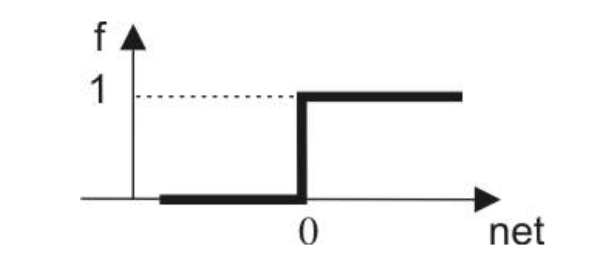
\includegraphics[width=8cm]{img/TLU.png}
\caption{Funkcija skoka}
\label{img:tlu}
\end{figure}

Znak nejednakosti u funkciji skoka, dodatno može u nekim slučajevima sadržavati i znak jednakosti čime se funkcija \ref{eq:tlu} mijenja u \ref{eq:linear-tlu}

\begin{equation}
f(net)=\left\{
\begin{array}{c l}	
     0   & $\textit{za net} $ \leq $ $ a,\\
     net & $\textit{za a} $ < $ \textit{net} $ < $ $ b,\\
     1   & $\textit{za net} $ \geq $ $ b
\end{array}\right.
\label{eq:Funkcija skoka koja je na dijelovima linearna}
\end{equation}

\begin{figure}[H]
\centering
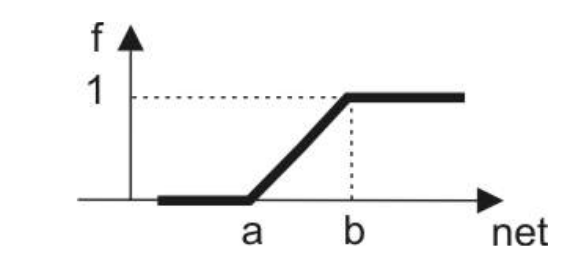
\includegraphics[width=8cm]{img/LinearTLU.png}
\caption{Na dijelovima linearna TLU}
\label{img:linear-tlu}
\end{figure}

Najčešća aktivacijska funkcija jest sigmoida. Vrlo važno svojstvo ove funkcije koje ju razlikuje od dosad navedenih funkcija jest da je derivabilna. To će se pokazati kao vrlo važna značajka za proces učenja neuronske mreže. Sigmoida je definirana kao:

\begin{equation}
f(net) = \frac{1}{1 + e^{-a net}}
\label{eq:sigmoid}
\end{equation}

\begin{figure}[H]
\centering
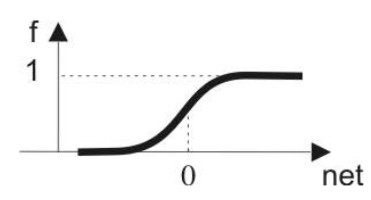
\includegraphics[width=8cm]{img/Sigmoid.png}
\caption{Sigmoidlana (logistička) funkcija}
\label{img:sigmoid}
\end{figure}

gdje parametar $a$ određuje nagib funkcije. Vrlo važno svojstvo sigmoide je da sve brojeve iz bilo kojeg intervala preslikava na raspon $[0,1]$. Zbog toga vrlo često izlaz iz logističke funkcije ima vjerojatnosnu interpretaciju, odnosno koristi se kada je na izlazu potrbno predvijeti vjerojatnosti. Važno je napomenuti da se sigmoida u području strojnog učenja koristi kada model ima binarni izlaz (predviđa 2 klase), dok se za višeklasnu regresiju/klasifikaciju koristi softmax:

\begin{equation}
f(net) = \frac{e^{net_i}}{\sum_{j=1}^{k} e^{net_j}}
\label{eq:sigmoid}
\end{equation}

\begin{figure}[H]
\centering
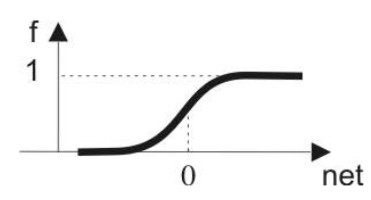
\includegraphics[width=8cm]{img/Sigmoid.png}
\caption{Sigmoidlana (logistička) funkcija}
\label{img:sigmoid}
\end{figure}

Softmax je generalizirana sigmoida. Izlaz iz funkcije softmax također vrlo često ima vjerojatnosnu interpretaciju. 

Zadnja aktivacijska funkcija koju ovdje valja spomenuti je ReLU (\textit{engl. Rectified Linear Unit}). 

\begin{equation}
f(net) = max(0, net)
\label{eq:relu}
\end{equation}

\begin{figure}[H]
\centering
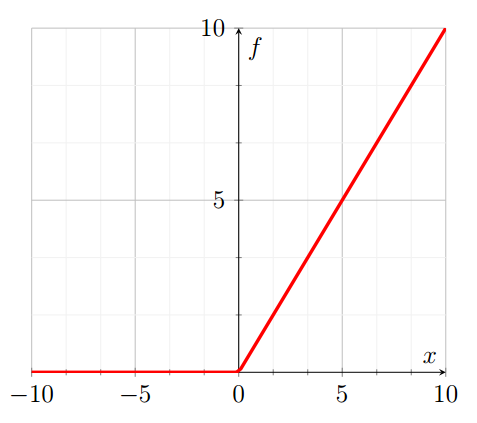
\includegraphics[width=8cm]{img/ReLU.png}
\caption{ReLU}
\label{img:relu}
\end{figure}

Ova aktivacijska funkcija je vrlo raširena u računalnom vidu i vrlo popularna kod konvolucijskih neuronskih mreža. Problem je što ova funkcija sve negativne vrijednosti stavlja u $0$ što smanjuje mogućmost modela da potpuno izvuče znanje iz podataka. Zato je osmišljena još jedna funkcija koja ne preslikava negativne vrijednosti u 0, nego u neku vrijednost blizu $0$ (što je vrijednost negativnija, preslikava se u vrijednost dalje od $0$). Ta funkcija naziva se "Leaky ReLU":

\begin{equation}
f(net)=\left\{
\begin{array}{c l}	
     a {net}   & $\textit{za net} $ < $ $ 0,\\
     {net}     & $\textit{za net} $ \geq $ $ 0
\end{array}\right.
\label{eq:Leaky ReLU}
\end{equation}

\begin{figure}[H]
\centering
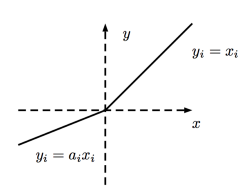
\includegraphics[width=8cm]{img/LeakyReLU.png}
\caption{Leaky ReLU}
\label{img:Leaky ReLU}
\end{figure}



sources: https://medium.com/the-theory-of-everything/understanding-activation-functions-in-neural-networks-9491262884e0
\section{Konvolucijske neuronske mreže}

Konvolucijske neuronske mreže mogu se zamisliti kao svojevrsno proširenje klasičnih višeslojnih neuronskih mreža. 

\chapter{Skupovi podataka}
\section{Pascal VOC2007}

Ovaj skup podataka \citep{pascal-voc-2007} također sadrži slike objekata u svakidašnjem okruženju. Ovdje se nalazi $9963$ slike sa $24 640$ objekata podijeljenih u $20$ kategorija:
\begin{itemize}
	\item \textbf{Person}: person
    \item \textbf{Animal}: bird, cat, cow, dog, horse, sheep
    \item \textbf{Vehicle}: aeroplane, bicycle, boat, bus, car, motorbike, train
    \item \textbf{Indoor}: bottle, chair, dining table, potted plant, sofa, tv/monitor
\end{itemize}
U ovom skupu podataka, slike su označene kao okviri (koordinate okvira).

\begin{figure}[h]
	\centering
	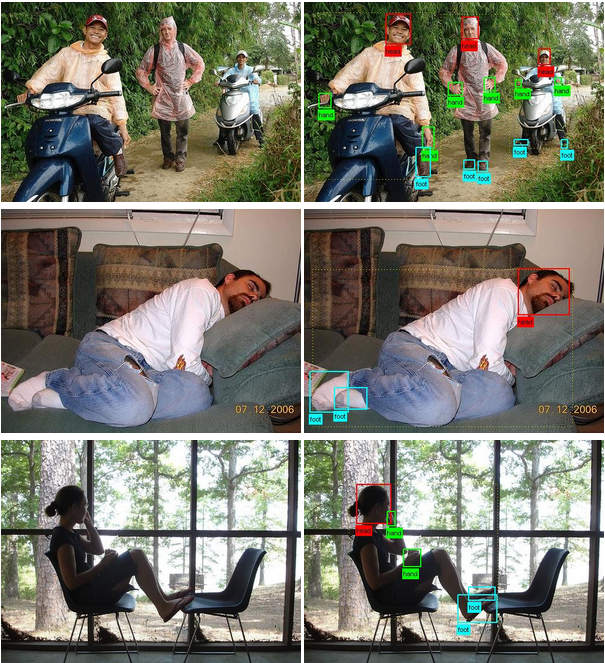
\includegraphics[width=9cm]{/home/luka/Workspaces/diplomski-rad/img/PascalVOC2007.png}
	\caption{Primjeri slika iz skupa Pascal VOC2007, \citep{pascal-voc-2007}}
	\label{img:pascalVOC2007}
\end{figure}

\section{COCO}

COCO (\textit{Common Object in Context}) \citep{coco} je skup podataka nastao 2014. godine. Kako i samo ime nalaže, COCO sadrži preko $330$ tisuća označenih slika sa $1.5$ milijuna označenih objekata u svakidašnjem okruženju i scenama te na taj način tim objektima pridružuje "kontekst". Ovaj skup podataka služi za treniranje algoritama čija je zadaća detekcija i klasifikacija objekata. COCO sadrži objekte podijeljene u $80$ klasa. Na slikama se nalazi više objekata od kojih su svi označeni i segmentirani tako da se na ovom skupu podataka može vršiti i trening mreže za segmentaciju slika. 

\begin{figure}[htp]
	\centering
	\begin{subfigure}[b]{0.4\linewidth}
		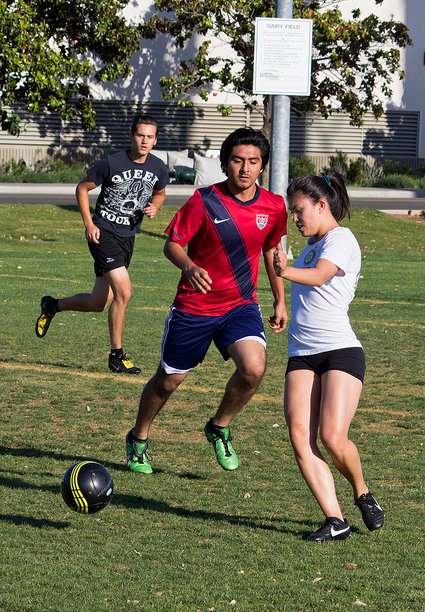
\includegraphics[width=\linewidth]{/home/luka/Workspaces/diplomski-rad/img/COCO1.png}
	\end{subfigure}
	\begin{subfigure}[b]{0.4\linewidth}
		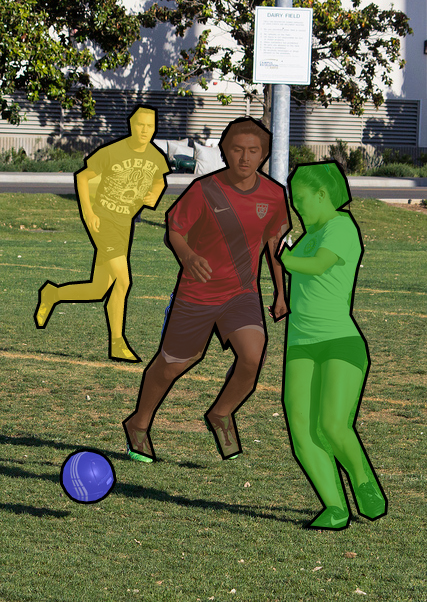
\includegraphics[width=\linewidth]{/home/luka/Workspaces/diplomski-rad/img/COCO11.png}
	\end{subfigure}
	\begin{subfigure}[b]{0.4\linewidth}
		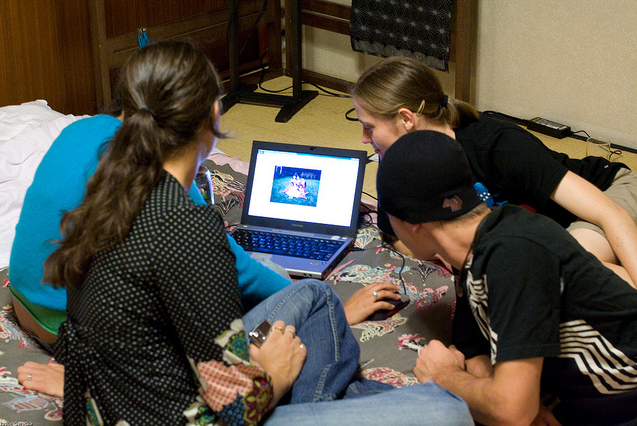
\includegraphics[width=\linewidth]{/home/luka/Workspaces/diplomski-rad/img/COCO2.png}
	\end{subfigure}
	\begin{subfigure}[b]{0.4\linewidth}
		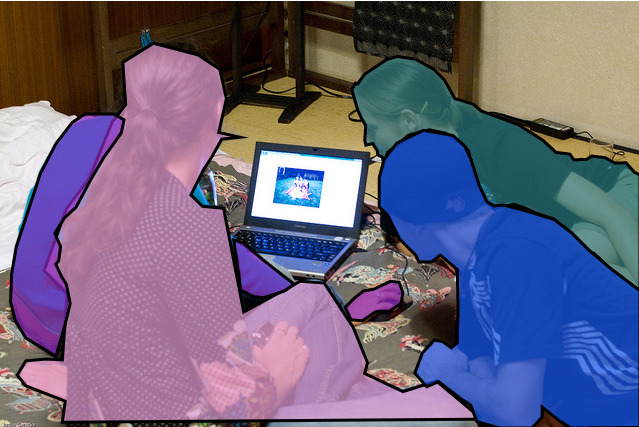
\includegraphics[width=\linewidth]{/home/luka/Workspaces/diplomski-rad/img/COCO22.png}
	\end{subfigure}
	\begin{subfigure}[b]{0.4\linewidth}
		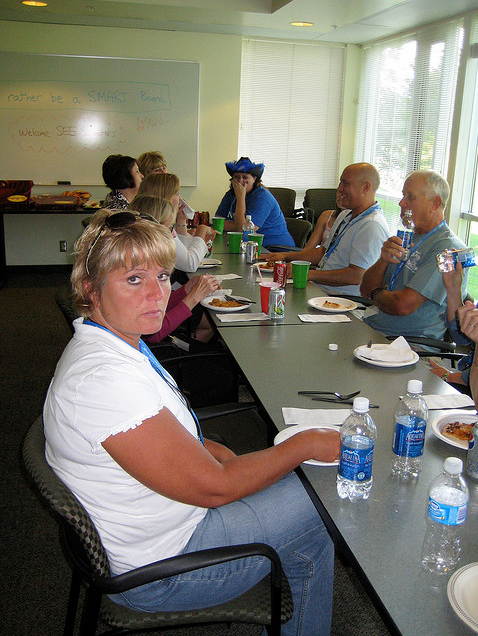
\includegraphics[width=\linewidth]{/home/luka/Workspaces/diplomski-rad/img/COCO3.png}
	\end{subfigure}
	\begin{subfigure}[b]{0.4\linewidth}
		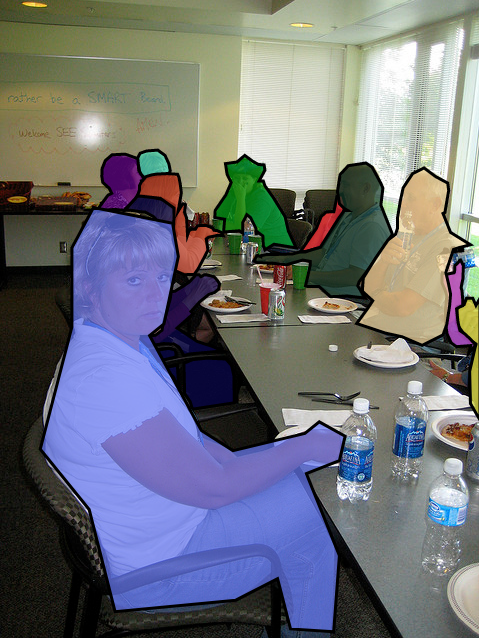
\includegraphics[width=\linewidth]{/home/luka/Workspaces/diplomski-rad/img/COCO33.png}
	\end{subfigure}
	\caption{Primjer slika i oznaka iz COCO skupa podataka, \citep{coco}}
	\label{img:coco-samples}
\end{figure}

\section{Video}

U ovom radu, istraživanje je provedeno na videu 'Esquina Democratica.mp4' preuzetom sa web lokacije: \textit{https://www.videezy.com/people/4966-people-and-commerce-in-a-street-one-point-perspective}. Ovaj video je rezolucije $1920x1080$ te sadrži 30 slika u sekundi videa (30 FPS).




\chapter{Implementacija}
Ovaj zadatak potrebno je razlomiti na nekoliko podzadataka:
\begin{itemize}
	\item detekcija osoba
	\begin{itemize}
		\item lokalizacija
		\item klasifikacija
	\end{itemize}
	\item praćenje objekata na videu
\end{itemize}


\section{Korišteni alati}

U ovom radu, algoritmi su implementirani u programskom jeziku \textbf{Python} verzije 3.6.5. na operacijskom sustavu Ubuntu Linux 18.04. Za konstrukciju neuronskih mreža korištena je biblioteka \textbf{Keras}. Keras je relativno nova biblioteka te je svojevrsna apstrakcija \textit{Tensorflow-a} jer pojednostavljuje konstrukciju mreže na način da se slojevi "sami brinu" o dimenzijama. Programer mora samo definirati ulaznu dimenziju podataka te izlaznu dimenziju. Ostalo biblioteka napravi sama. Iz tog razloga je vrlo popularna te je primarno namjenjena brzom prototipiziranju mreža, dok su performanse u drugom planu. U Kerasu, autor može birati nekoliko biblioteka za neuronske mreže koje u pozadini odrađuju posao kao što su \textbf{Tensorflow}, \textbf{CNTK} i \textbf{Theano}. U implementaciji se u pozadini koristi \textbf{Tensorflow}. Keras u pozadini koristi i standardne biblioteke kao što su \textit{NumPy, Scipy} i sl. za numeričke i ostale operacije. Za Viola-Jones algoritam, kao i učitavanje slika i videa, spremanje i crtanje okvira korištena je biblioteka \textit{OpenCV}.
\section{Viola-Jones algoritam}

Kao primjer algoritama za detekciju objekata implementiran je i algoritam Viole i Jonesa opisan u poglavlju 3.2. Algoritam je implementiran korištenjem biblioteke \textit{OpenCV}.

Algoritam prima nekoliko ulaznih parametara od kojih je obavezan samo parametar "- -video" kojim se zadaje video na kojem da se vrši detekcija i praćenje osoba. Parametar "- -win-stride" je uređeni par vrijednosti $(x, y)$ koji određuje korak u smijeru $x$ i $y$ osi po kojima se kreće klizeći prozor. Zadana vrijednost je $(8, 8)$. Idući bitan parametar je "--scale". Ovaj parametar omogućuje detekciju ljudi različitih veličina na slici (i ljudi koji su blizu i ljudi koji su daleko). Povećanjem ovog parametra povećava se i rizik da ne budu detektirani svi objekti, ali istovremeno se algoritam i ubrzava. Obrnuto, smanjenjem ovog parametra algoritam detektira više objekata i usporava mu se rad. Posljedično, javlja se i više false-positiva. U implementaciji je ovaj algoritam postavljen na vrijednost $1.05$. Ostavljena je i mogućnost spremanja svake slike u videu (svakog \textit{framea}) parametrom "- -save" radi kasnije evaluacije. 

\begin{figure}[htp]
	\centering
	\includegraphics[width=9cm]{/home/luka/Workspaces/diplomski-rad/img/ViolaJonesFrames/frame_3.png}
	\caption{Primjer detekcije Viola-Jones algoritmom}
	\label{img:violaJones-detection-example}
\end{figure}

\section{YOLO}

U okviru ovog rada implementiran je i algoritam za detekciju objekata pod nazivom \textbf{YOLO - You Only Look Once} \citep{YOLO}. Ovaj algoritam je predvodnik novih revolucionarnih algoritama za detekciju objekata. Trenutno najnovija, treća, verzija ovog algoritma nastala je 2018. godine, dok se algoritam, u svojoj osnovnoj inačici, pojavio 2015. godine. Također, postoje dvije inačice svake verzije algoritma: \textit{full-YOLO} i \textit{tiny-YOLO}. Tiny-YOLO ima manju mrežu i, naravno, slabije sposobnosti, no ima bolje performanse. 

Prije ovog algoritma, detekcija objekata se vršila pomoću klasifikatorskih ili lokalizacijskih mreža. Takve mreže primjenjuju se na različita područja slike te na različito skaliranu sliku. One regije slike za koje su mreže vrlo sigurne smatraju se detekcijom. YOLO algoritam koristi potpuno novu paradigmu, novi pristup detekciji objekata. Ideja je da se kroz mrežu provuće jedna slika, bez skaliranja ili dovođenja različitih regija slike na ulaz mreže. Dakle, postupak detekcije objekata u mreži YOLO jest da mreža sama podijeli sliku na regije te predviđa okvire objekata (\textit{engl. bounding-box}) te njihove vjerojatnosti za svaku regiju. Odnosno, klasifikacija i lokalizacija objekata na slici te predviđanje okvira objekata su sve zadaće jedne mreže. 

\subsection{Dizajn i svojstva mreže}

U tablici \ref{tab:yolo_architecture} prikazana je arhitektura mreže Yolo. Radi preglednosti tablice, pod slojem Conv podrazumijeva se konvolucijski sloj dimenzija kako su napisane, Batch Normalization sloj koji, kako mu samo ime kaže, služi na normalizaciju \textit{batcha}, poboljšava konvergenciju modela dok istovremeno služi i kao regularizator. Na kraju je dodan i Leaky ReLu sloj.

\begin{minipage}{\linewidth}
\centering

\begin{tabular}{||l|l|l|l|l||}
\hline
	Ime sloja & Filteri & Korak & Dimenzije na ulazu & Dimenzije na izlazu \\
\hline
	Conv1 & 3 x 3 x 32 & 1 x 1 & 416 x 416 x   3 & 416 x 416 x  32 \\
\hline
	MaxPool1 & 2 x 2 & 2 x 2 & 416 x 416 x  32 & 208 x 208 x  32 \\
\hline
	Conv2 & 3 x 3 x 64 & 1 x 1 & 208 x 208 x  32 & 208 x 208 x  64 \\
\hline
	MaxPool2 & 2 x 2 & 2 x 2 & 208 x 208 x  64 & 104 x 104 x  64 \\
\hline
	Conv3 & 3 x 3 x 128 & 1 x 1 & 104 x 104 x  64 & 104 x 104 x 128 \\
\hline	
	Conv4 & 1 x 1 x 64 & 1 x 1 & 104 x 104 x 128 & 104 x 104 x  64 \\
\hline
	Conv5 & 3 x 3 x 128 & 1 x 1 & 104 x 104 x  64 & 104 x 104 x 128 \\
\hline
	MaxPool2 & 2 x 2 & 2 x 2 & 104 x 104 x 128 & 52 x  52 x 128 \\
\hline
	Conv6 & 3 x 3 x 256 & 1 x 1 & 52 x  52 x 128 & 52 x  52 x 256 \\
\hline
	Conv7 & 1 x 1 x 128 & 1 x 1 & 52 x  52 x 256 & 52 x  52 x 128 \\
\hline
	Conv8 &  3 x 3 x 256 & 1 x 1 & 52 x  52 x 128 & 52 x  52 x 256 \\
\hline
	MaxPool3 & 2 x 2 & 2 x 2 & 52 x  52 x 256 & 26 x  26 x 256 \\
\hline
	Conv9 & 3 x 3 x 512 & 1 x 1 & 26 x  26 x 256 & 26 x  26 x 512 \\
\hline
	Conv10 & 1 x 1 x 256 & 1 x 1 & 26 x  26 x 512 & 26 x  26 x 256 \\
\hline
	Conv11 & 3 x 3 x 512 & 1 x 1 & 26 x  26 x 256 & 26 x  26 x 512\\
\hline
	Conv12 & 1 x 1 x 256 & 1 x 1 & 26 x  26 x 512 & 26 x  26 x 256 \\
\hline
	Conv13 & 3 x 3 x 512 & 1 x 1 & 26 x  26 x 256 & 26 x  26 x 512 \\
\hline
	MaxPool4 & 2 x 2 & 2 x 2 & 26 x  26 x 512 & 13 x  13 x 512 \\
\hline
	Conv14 & 3 x 3 x 1024 & 1 x 1 & 13 x  13 x 512 & 13 x  13 x 1024 \\
\hline
	Conv15 & 1 x 1 x 512 & 1 x 1 & 13 x  13 x 1024 & 13 x  13 x 512 \\
\hline
	Conv16 & 3 x 3 x 1024 & 1 x 1 & 13 x  13 x 512 & 13 x  13 x 1024 \\
\hline
	Conv17 & 1 x 1 x 512 & 1 x 1 & 13 x  13 x 1024 & 13 x  13 x 512 \\
\hline
	Conv18 & 3 x 3 x 1024 & 1 x 1 & 13 x  13 x 512 & 13 x  13 x 1024 \\
\hline
	Conv19 & 3 x 3 x 1024 & 1 x 1 & 13 x  13 x 1024 & 13 x  13 x 1024 \\
\hline
	Conv20 & 3 x 3 x 1024 & 1 x 1 & 13 x  13 x 1024 & 13 x  13 x 1024 \\
\hline
\hline
	Route & from & Conv13 & & \\
\hline
	Conv21 & 1 x 1 x 64 & 1 x 1 & 26 x  26 x 512 & 26 x  26 x  64 \\
\hline
\hline
	Space2Depth & reshape & & & \\
\hline
	Concatenate & Route from Conv20 & and & Space2Depth & \\
\hline
	Conv22 & 3 x 3 x 1024 & 1 x 1 & 13 x  13 x 1280 & 13 x  13 x 1024 \\
\hline
	Conv23 & 1 x 1 x 425 & 1 x 1 & 13 x  13 x 1024 & 13 x  13 x 425 \\
\hline
\hline
\end{tabular}
\captionof{table}{Yolo arhitektura} \label{tab:yolo_architecture} 
\end{minipage}

\subsection{Podjela slike}
\label{cells-section}

Kada se na ulaz mreže dovede slika, prva stvar koju mreža napravi jest da podijeli sliku u \textbf{C} x \textbf{C} ćelija kao što to prikazuje slika \ref{img:yolo_grid_cells}. Svaka od tih ćelija predviđa točno \textbf{jedan} objekt. Primjerice, žuta ćelija na slici pokušava predvidjeti objekt klase osoba čiji se centar (plava točka na slici desno) nalazi unutar te čelije.

\begin{figure}[htp]
	\centering
	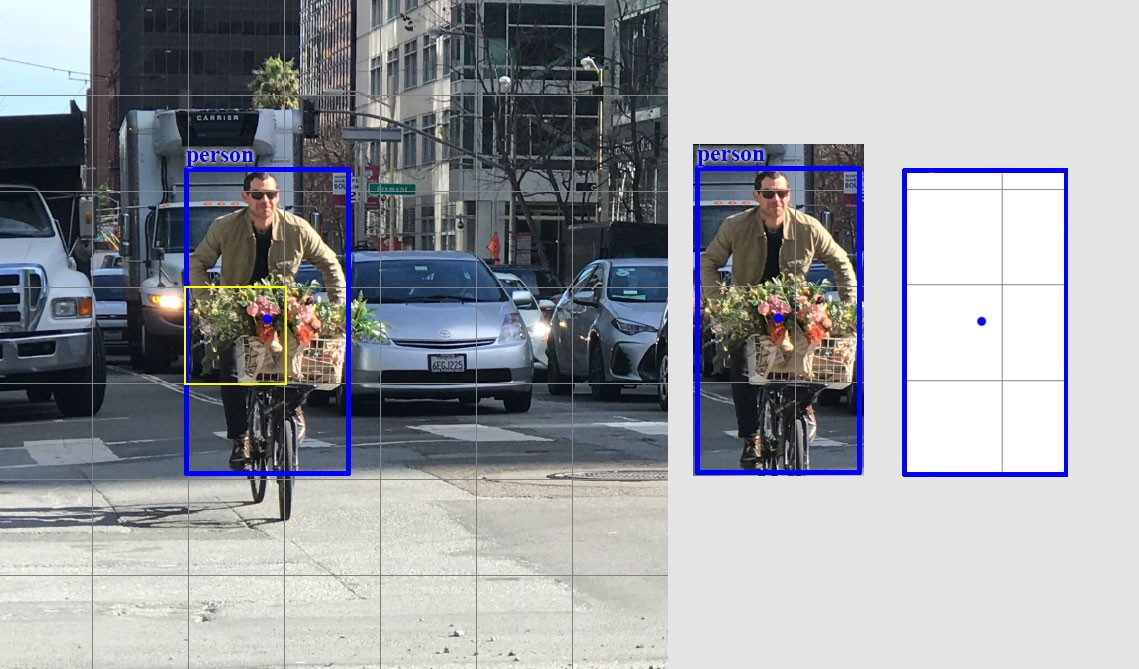
\includegraphics[width=10cm]{/home/luka/Workspaces/diplomski-rad/img/Yolo_grid.jpeg}
	\caption{Podijela slike na \textbf{C} x \textbf{C} ćelija}
	\label{img:yolo_grid_cells}
\end{figure}

Svaka ćelija predviđa fiksan broj okvira (\textit{engl. bounding boxes}. Na slici \ref{img:bounding_boxes} žuta ćelija predviđa dva okvira kako bi locirala osobu na slici. 

\begin{figure}[htp]
\centering
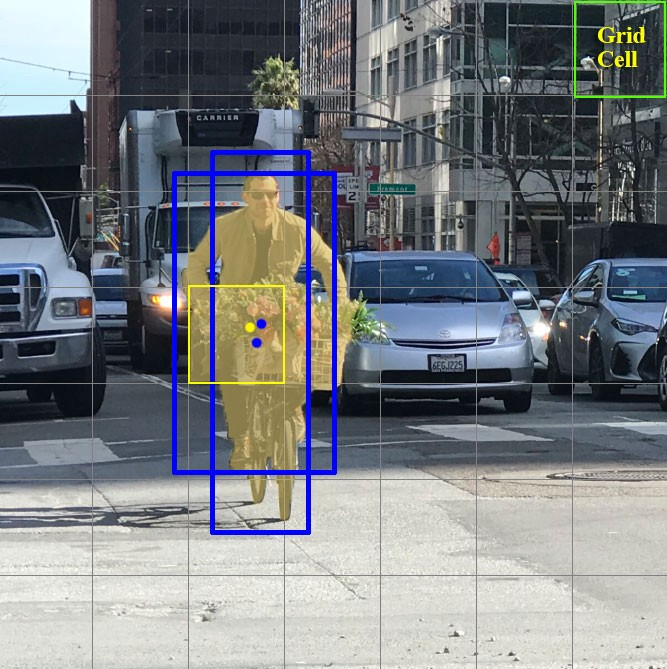
\includegraphics[width=10cm]{/home/luka/Workspaces/diplomski-rad/img/Yolo_cell_boxes.jpeg}
\caption{Predviđanje okvira}
\label{img:bounding_boxes}
\end{figure}

Međutim, mogućnost predviđanja samo jednog objekta po čeliji donekle ograničava algoritam u smislu blizine objekata koje može detektirati. Odnosno, ako se u čeliji nalazi više od 1 objekta, algoritam mora odabrati samo 1 koji od njih koji će detektirati.  

Za svaku čeliju \textbf{C} algoritam predviđa:
\begin{itemize}
	\item \textbf{B} okvira te za svaki okvir njegovu pouzadnost (\textit{engl. box confidence score})
	\item samo jedan objekt
	\item \textbf{P} vjerojatnosti, po jednu za svaku klasu \textbf{C}
\end{itemize}

Ulaz u mrežu može biti proizvoljne veličine, no mreža YOLO preoblikuje ulaz u dimenzije $416\times416\times3$ kako bi ga mogao dovesti na ulaz u mrežu. Mreža dijeli sliku na $13\times13$ ćelija. Svaka ćelija predviđa 5 okvira za objekt koji se nalazi u toj čeliji (ako se nalazi), te svaki od okvira ima 85 parametara. Izlaz iz mreže je oblika $(13, 13, 425)$. U svrhu razumijevanja izlaza iz mreže, zgodno ga je zamisliti kao kompozit tri tenzora:

\begin{itemize}
	\item pouzdanost okvira \textit{(engl. box\_confidence)} kao tenzor dimenzije $(13\times13, 5, 1)$ koji sadrži $p_c$ pouzdanost postojanja objekta u svakom od 5 predviđenih okvira u čeliji \textbf{C} za svaku od $13\times13$ ćelija
	\item okviri \textit{(engl. boxes)} kao tenzor dimenzije $(13\times13, 5, 4)$ koji sadrži $(x_{top}, y_{top}, x_{bottom}, y_{bottom})$ za svaki od 5 okvira u čeliji
	\item vjerojatnosti klasa za okvire \textit{(engl. box\_class\_prob)} kao tenzor dimenzije $(13\times13, 5, 80)$ koji čuva informaciju o pouzdanosti za svaku od 80 klasa za svaki od 5 okvira u čeliji.
\end{itemize}

\begin{figure}[htp]
	\centering
	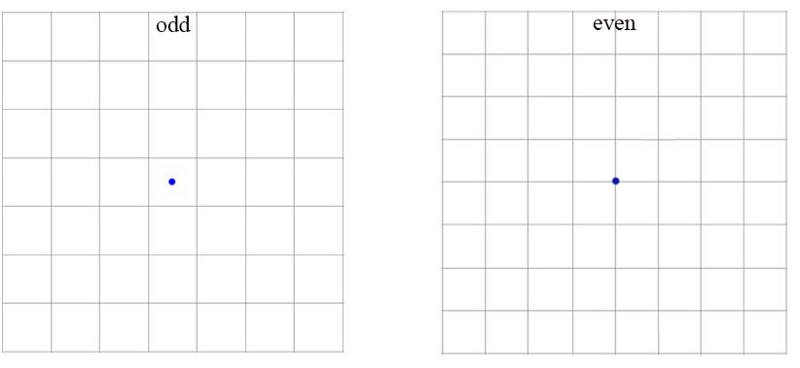
\includegraphics[width=8 cm]{/home/luka/Workspaces/diplomski-rad/img/yolo_grid.jpeg}
	\caption{Neparan i paran broj ćelija po dimenziji}
	\label{img:yolo-grid}
\end{figure}

Kao što prikazuje slika \ref{img:yolo-grid}, neparan broj ćelija po dimenziji (npr. $13\times13$) je pogodan jer je jednostavnije odrediti u kojoj se čeliji objekt nalazi.

\subsection{Funkcija gubitka}

Yolo algoritam predviđa više okvira po jendoj čeliji na slici. Od svih tih ćelija, potrebno je zadržati samo one u kojima se zaista nalazi objekt. U tu svrhu, izabire se ona ćelija koja ima naveći IoU (\textit{engl. Intersection over Union}) sa stvarnim objektom (\textit{engl. ground truth}). Za računanje gubitka, Yolo koristi sumu kvadrata pogrešaka predviđanja algoritma i stvarnih objekata. Zbog ideje Yolo algoritma da se klasifikacija i lokalizacija rade istom mrežom u jednom prolasku, funkcija gubitka sastavljena je od nekoliko dijelova.

\begin{figure}[htp]
	\centering
	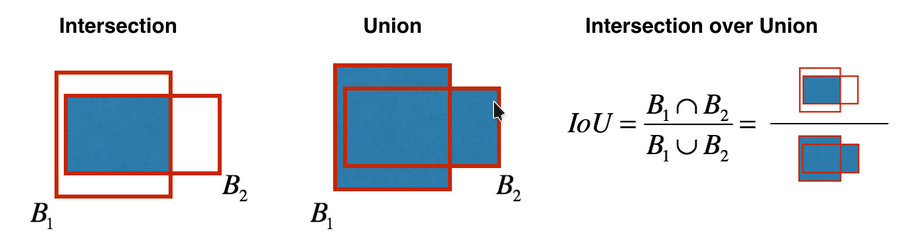
\includegraphics[width=11cm]{/home/luka/Workspaces/diplomski-rad/img/IoU.png}
	\caption{Intersection over union}
	\label{img:IoU}
\end{figure}

\begin{itemize}
	\item{\textbf{Pogreška klasifikacije}}
	
	Ako je objekt detektiran, pogreška klasifikacije u svakoj čeliji računa se kao kvadrat pogreške uvjetne vjerojatnosti za svaku klasu.
	
	\begin{equation}
		\centering
		\sum_{i=1}^{S\times S} 1_i^{obj} \sum_{c \in klase} (p_i(c) - \hat{p}_i(c))^2
		\label{eq:classification-loss}
	\end{equation}
	
	gdje 
	\begin{itemize}
		\item $1_i^{obj} = 1$ ako se objekt pojavljuje u čeliji i, inače $0$
		\item $\hat{p}_i(c)$ označava uvjetnu vjerojatnost klase $c$ u čeliji $i$
	\end{itemize}
	
	\item{\textbf{Pogreška lokalizacije}}
	
	Ovaj segment funkcije pogreške mjeri grešku u lokaciji i veličini predviđenih okvira. U obzir se uzimaju samo oni okviri u kojima se objekt nalazi. Ideja je da se jednaka greška u velikom i u malom predviđenom okviru ne kažnjavaju jednako (npr. greška od 2px u velikom i malom okviru). Zbog toga Yolo predviđa \textbf{korjene kvadrata} visine i širine okvira. Nadalje, kako bi još točije predviđao okvire, pogreška okvira se množi paramterom $\lambda_{coord}$.
	
	\begin{align}
		\centering
		\begin{split}
			\lambda_{coord}\sum_{i=0}^{S^2}\sum_{j=0}^{B} 1_{ij}^{obj} [(x_i - \hat{x}_i)^2 + (y_i - \hat{y}_i)^2] + \\
			\lambda_{coord}\sum_{i=0}^{S^2}\sum_{j=0}^{B} 1_{ij}^{obj} [(\sqrt{w_i} - \sqrt{\hat{w}_i})^2 + (\sqrt{h_i} - \sqrt{\hat{h}_i})^2]
		\end{split}
		\label{eq:localization-loss}
	\end{align}
	
	gdje 
	\begin{itemize}
		\item $1_{ij}^{obj} = 1$ ako se objekt nalazi u $j$-tom okviru $i$-te ćelije, inače $0$
		\item $\lambda_{coord}$ parametar za ugađanje težine za pogrešku u koordinatama okvira
	\end{itemize}
	
	\item{\textbf{Pogreška pouzdanosti}}

	Ovdje se javljaju dva slučaja:
	\begin{enumerate}
		\item \textbf{Objekt je detektiran u okviru}
		
		\begin{equation}
			\centering
			\sum_{i=0}^{S^2}\sum_{j=0}^{B} 1_{ij}^{obj} (C_i - \hat{C}_i)^2
			\label{eq:confidence-loss-1}
		\end{equation}
		
		gdje 
		\begin{itemize}
			\item $1_{ij}^{obj} = 1$ ako se objekt nalazi u $j$-tom okviru $i$-te ćelije, inače $0$
			\item $\hat{C}_i$ jest iznos pouzdanosti za okvir $j$ u čeliji $i$
		\end{itemize}
		
		\item \textbf{Objekt nije detektiran u okviru}
		
		Večina okvira ne sadrži objekt što dovodi do problema neravnomjernosti klasa, odnosno, model se trenira da puno češće detektira pozadinu nego sami objekt. Kako bi se ovaj problem riješio, gubitak se množi faktorom $\lambda_{no-obj}$ koji ima vrijednost između $0$ i $1$.
		
		\begin{equation}
			\centering
			\lambda_{no-obj}\sum_{i=0}^{S^2}\sum_{j=0}^{B} 1_{ij}^{no-obj} (C_i - \hat{C}_i)^2
			\label{eq:confidence-loss-2}
		\end{equation}
		
		gdje 
		\begin{itemize}
			\item $1_{ij}^{no-obj}$ jest komplement gornjeg izraza $1_{ij}^{obj}$
			\item $\hat{C}_i$ jest iznos pouzdanosti za okvir $j$ u čeliji $i$
			\item $\lambda_{no-obj}$ je faktor kojim se smanjuje iznos gubitka pri detekciji pozadine
		\end{itemize}
		
	\end{enumerate}	
		
\end{itemize}

\subsection{Anchor boxes}
\label{anchor-boxes-section}

\begin{figure}[htp]
	\centering
	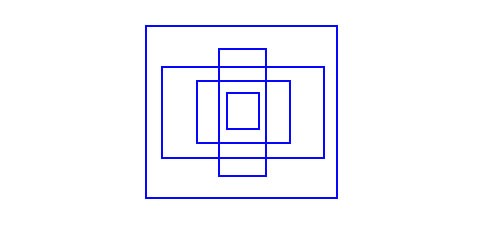
\includegraphics[width=8cm]{/home/luka/Workspaces/diplomski-rad/img/Anchor_boxes_img.jpeg}
	\caption{Klasteri dimenzija za anchor boxeve}
	\label{img:anchor-boxes}
\end{figure}

\textit{Anchor boxes} ili \textit{priors} jest još jedan pojam uveden ovim algoritmom. Kako u početku treninga mreža ne bi predviđala okvire nasumično, predloženo je da se, ovisno o domeni i podacima, izabere $n$ najčešćih okvira koji najbolje opisuju klase u tom skupu podataka. Primjerice, pješake se uglavnom može označiti uspravnim pravokutnim okvirom, dok je kod automobila okvir obično polegnuti pravokutnik. Na ovaj način uzeto je 5 standardnih okvira (\textit{anchor boxes}) koji su izračunati K-means klusteringom ($k=5$) iz COCO i VOC2007 skupova podataka kako bi se pronašle centoride $k$ najboljih klastera. Da bi se odredile točne dimenzije standardnih okvira, korišena je IoU mjera. Izračunati anchor boxevi prikazani su slikom \ref{img:yolo-anchors}. Ljubičasti okviri uzeti su iz COCO skupa podataka, a bijeli sa crnim rubom iz VOC2007 skupa podataka.

\begin{figure}[htp]
	\centering
	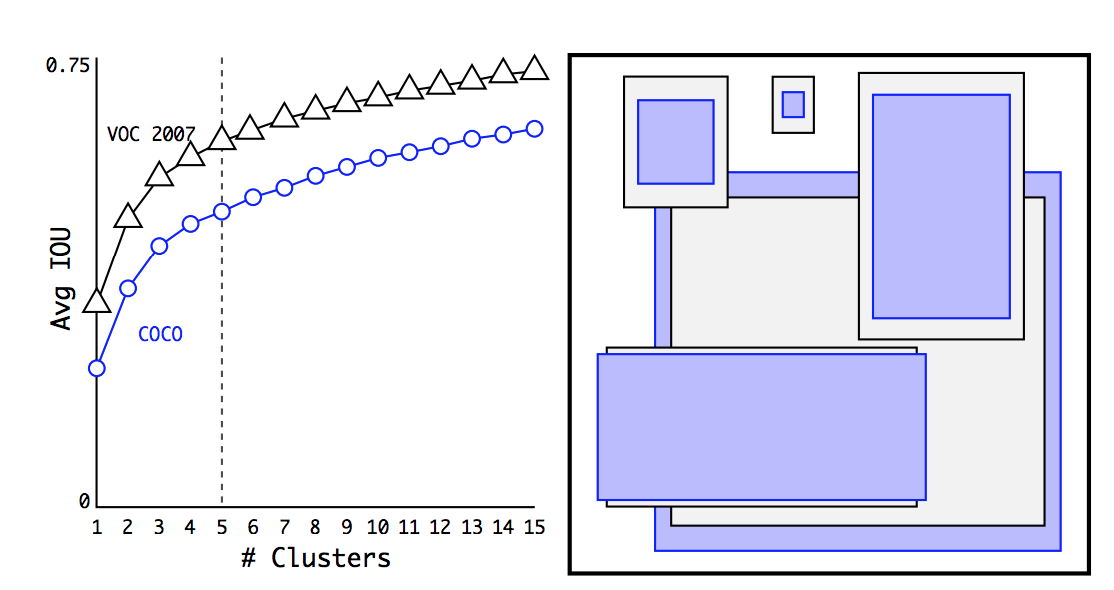
\includegraphics[width=9cm]{/home/luka/Workspaces/diplomski-rad/img/Yolo_anchor_boxes.png}
	\caption{Standardni okviri dobiveni K-means klasteringom i IoU mjerom \citep{YOLO}}
	\label{img:yolo-anchors}
\end{figure}

Tako sada Yolo mreža predviđa koordinate okvira objekta direktno, no relativno u odnosu na pozicuju promatrane ćelije od gornjeg lijevog ruba. Nadalje, okviri se predviđaju kao odstupanje od nekog od standardnih okvira. To odstupanje je ograničeno kako nebi bilo koji okvir mogao prijeći u bilo koji drugi jer se onda gubi smisao ovog cijelog postupka. Ograničavanjem odstupanja omogućeno je kako bi se svako predviđanje moglo opredjeliti za točno jedan oblik iz skupa standardnih okvira.

\subsection{Backbone}

Mreža kojom se inicijalizira Yolo mreža naziva se \textit{DarkNet} \citep{Darknet}. Mreža je prikazana na slici \ref{img:darknet}

\begin{figure}[htp]
	\centering
	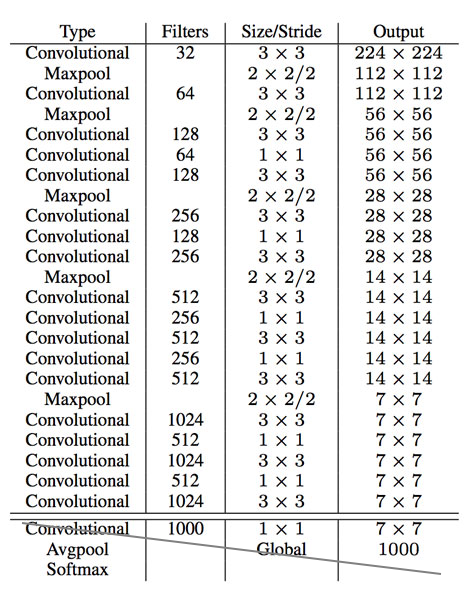
\includegraphics[width=8cm]{/home/luka/Workspaces/diplomski-rad/img/Darknet.png}
	\caption{Originalna DarkNet-19 mreža \citep{YOLO}}
	\label{img:darknet}
\end{figure}

Zadnji slojevi (koji su prekriženi na slici \ref{img:darknet}) izbačeni su za potrebe Yolo mreže. Ova arhitektura zahtjeva oko 5.8 milijardi operacija što je, u usporedbi sa VGG16 mrežom koja ima 3 sloja manje i zahtjeva oko 30.69 milijardi operacija za samo jednu sliku veličine $224 \times 224$, izuzetno malo i efikasno.

\subsection{Trening}

Prvo se trenira mreža DarkNet-19 za klasifikaciju na ImageNet skupu podataka sa 1000 klasa objekata u 160 epoha koristeći stohastički gradijentni spust (\textit{SGD}). Stopa učenja inicijalno je postavljena na vrijednost $0.1$ sa polinomijalnim raspadom potencije $4$, \textit{weight decay} parametrom postavljenim na $0.0005$ te momentom vrijednosti $0.9$. Tijekom treninga koriste se standardne metode izmjene podataka kao što su nasumično izrezivanje, rotacija i izmjene boje.

Zatim se izgradi mreža YOLO, prenesu se težine iz DarkNet mreže u početne slojeve mreže YOLO, te se ponovo trenira. Stopa učenja kreće od vrijednosti $10^{-3}$, a smanjuje se nakon 10, 60 i 90 epoha na isti način kao i kod treniranja DarkNeta. Parametar \textit{weight decay} postavljen je na vrijednost od $0.0005$, a moment na vrijednost $0.9$. Koriste se i metode izmjene boja, nasumičnog izrezivanja itd. kako bi algoritam bio što robusniji. Mreža se na taj način trenira na COCO i VOC2007 skupovima podataka.

Yolo mreža može primati slike različitih veličina. Svakih 10 \textit{batcheva} algoritam nasumično odabere neku veličinu slike za treniranje modela (veličina slike mora biti višekratnik broja $32$). Na taj način, prisiljava se mrežu da predviđa dobro za slike različitih dimenzija i skala. Na taj način omogućava se prilagodba mreže za određenu svrhu. Primjerice, ako je potrebno raditi predviđanja u stvarnom vremenu, moguće je davati manje slike algoritmu kako bi predviđanja bila brža. Ako je pak cilj da predviđanja budu što točnija, mogu se uzimati slike veće rezolucije.

\subsection{Predviđanje}

Način na koji YOLO detektira objekte i predviđa okvire objašnjeni su u podpoglavljima \ref{cells-section} i \ref{anchor-boxes-section}. No još nije spomenuto na koji način YOLO zaključuje koje okvire treba odbaciti a koje zadržati. Dakle, za neki objekt mreža predvidi nekoliko okvira. Metoda kojom se odabiru okviri za odbacivanje naziva se \textbf{Non-Maximal Suppression}. Način na koji ta metoda radi jest da poreda okvire po pouzdanosti, iterira kroz njih i odbacuje sve okvire koji predviđaju istu klasu kao neki od prethodnih i imaju IoU veći od $0.5$ sa tim prethodnim okvirom iste klase. Taj proces se ponavlja dok svi okviri ne budu ili odbačeni ili zadržani.

\begin{figure}[htp]
	\centering
	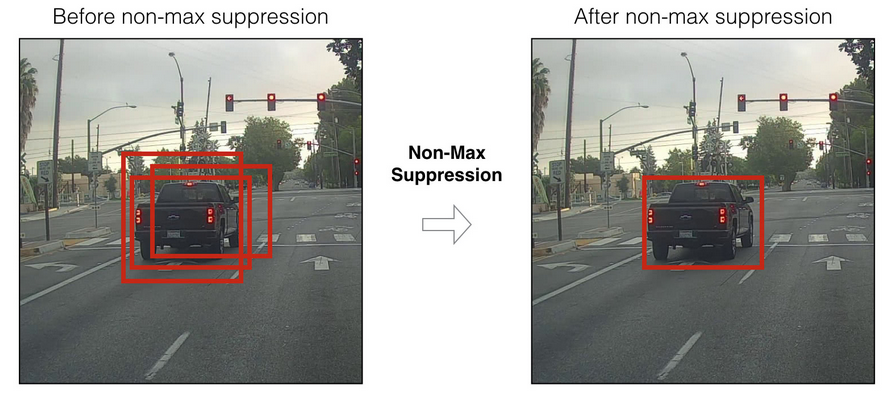
\includegraphics[width=10cm]{/home/luka/Workspaces/diplomski-rad/img/NMS.png}
	\caption{Non-Maximal Suppression}
	\label{img:nms}
\end{figure}

\chapter{Eksperimentalni rezultati}
Postoje dvije vrste podataka na kojima je moguće provesti ovo istraživanje: slika i video. Nije potrebno navoditi da koristeći sliku, zbog svojstva statičnosti, eliminiramo zadatak praćenja objekata.

\section{Viola-Jones algoritam}

Algoritam Viole i Jones-a, iako osmišljen davno, koristi se i danas. Izuzetno je brz, dovoljno točan i zahtjeva malo računalnih resursa. Sami algoritam opisan je u poglavlju 3.2. 

\begin{figure}[htp]
	\centering
	\begin{subfigure}[b]{0.4\linewidth}
		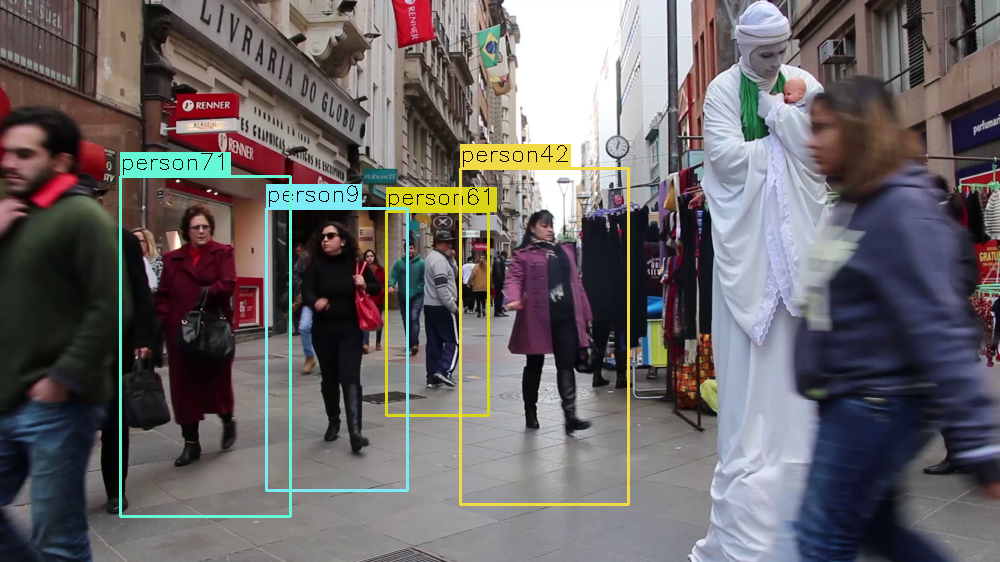
\includegraphics[width=\linewidth]{/home/luka/Workspaces/diplomski-rad/img/frame_0.png}
	\end{subfigure}
	\begin{subfigure}[b]{0.4\linewidth}
		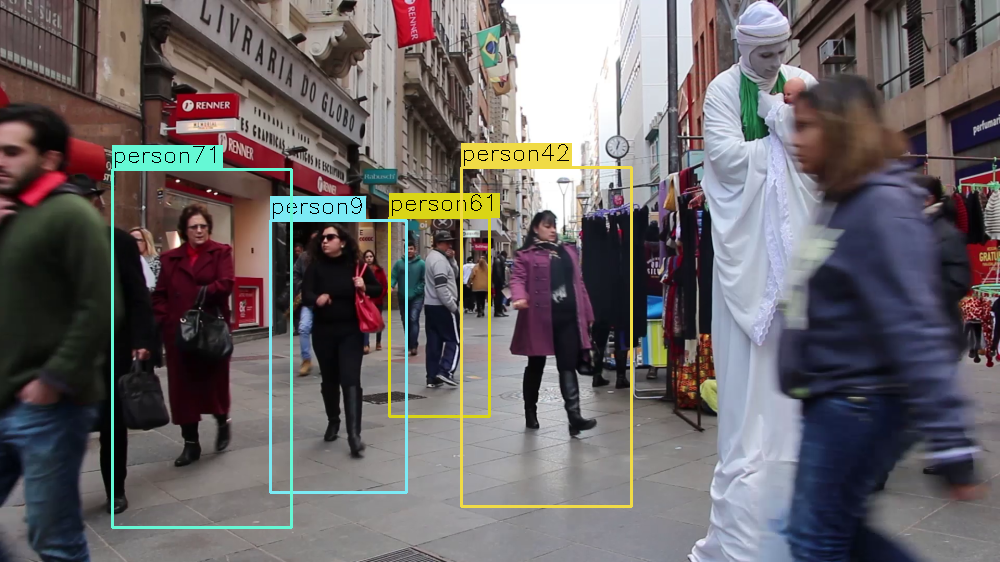
\includegraphics[width=\linewidth]{/home/luka/Workspaces/diplomski-rad/img/frame_1.png}
	\end{subfigure}
	\begin{subfigure}[b]{0.4\linewidth}
		\includegraphics[width=\linewidth]{/home/luka/Workspaces/diplomski-rad/img/frame_3.png}
	\end{subfigure}
	\begin{subfigure}[b]{0.4\linewidth}
		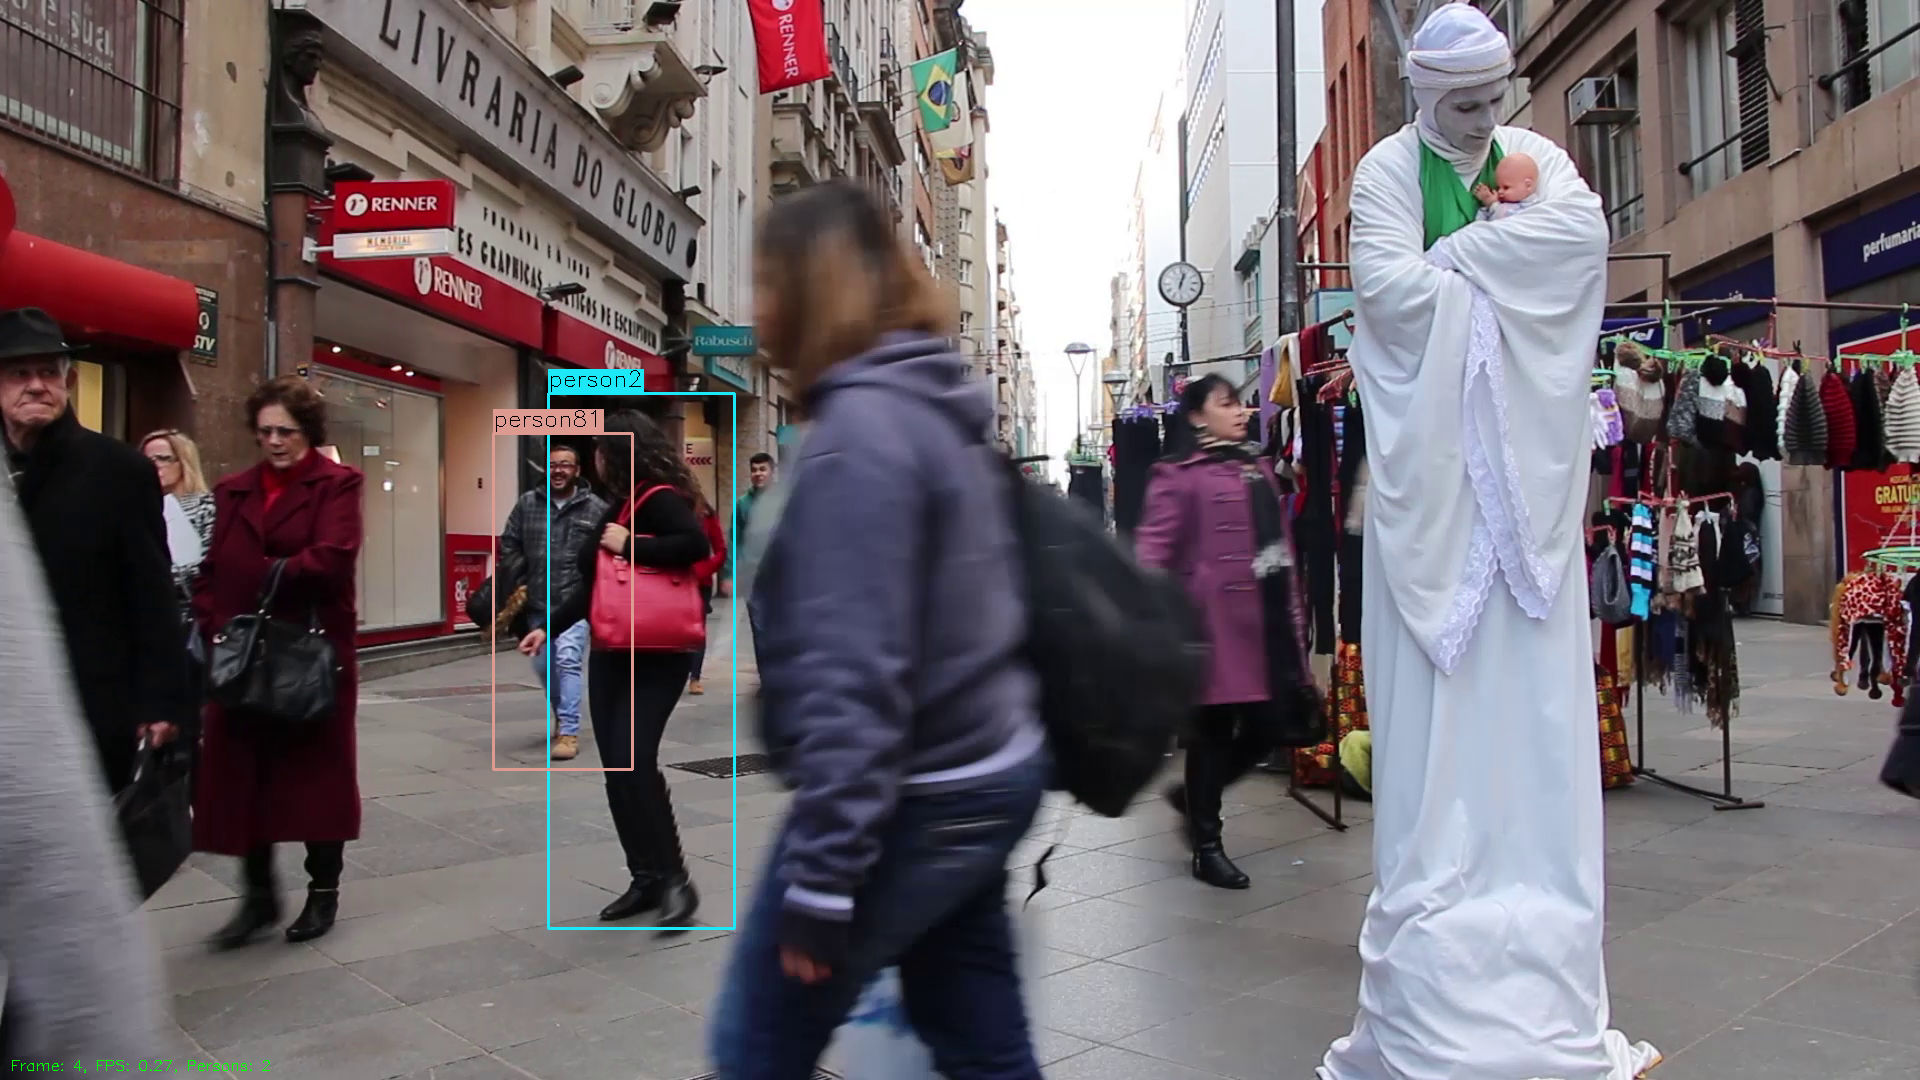
\includegraphics[width=\linewidth]{/home/luka/Workspaces/diplomski-rad/img/frame_4.png}
	\end{subfigure}
	\caption{Primjer detekcije Viola-Jones algoritmom}
	\label{img:violaJones-detection}
\end{figure}

Viola-Jones algoritam vrlo je pouzdan i dolazi sa većinom biblioteka specijaliziranih za računalni vid (\textit{OpenCV}). Za razliku od YOLO-a, ovaj algoritam ima nešto više false-positivea. Nekoliko slika sa pogrešnim označavanjem prikazano je na slici \ref{img:violaJones-fp}. Još jedan od nedostataka ovog algoritma jest osjetljivost na različite fotometrijske značajke (promjene svijetlosti). 

\begin{figure}[htp]
	\centering
	\begin{subfigure}[b]{0.4\linewidth}
		\includegraphics[width=\linewidth]{/home/luka/Workspaces/diplomski-rad/img/ViolaJonesFrames/frame_5.png}
	\end{subfigure}
	\begin{subfigure}[b]{0.4\linewidth}
		\includegraphics[width=\linewidth]{/home/luka/Workspaces/diplomski-rad/img/ViolaJonesFrames/frame_7.png}
	\end{subfigure}
	\begin{subfigure}[b]{0.4\linewidth}
		\includegraphics[width=\linewidth]{/home/luka/Workspaces/diplomski-rad/img/ViolaJonesFrames/frame_11.png}
	\end{subfigure}
	\begin{subfigure}[b]{0.4\linewidth}
		\includegraphics[width=\linewidth]{/home/luka/Workspaces/diplomski-rad/img/ViolaJonesFrames/frame_17.png}
	\end{subfigure}
	\caption{Primjer detekcije Viola-Jones algoritmom}
	\label{img:violaJones-detection}
\end{figure}

\section{YOLO}

Ovaj je algoritam, u originalnom obliku, implementiran u programskom jeziku C te je izuzetno brz. U radu se spominje da na grafičkoj kartici NVidia Titan X postiže brzine od 45 do 90 FPS (\textit{engl. Frames Per Second}) što je izuzetno brzo, uzimajući u obzir i izvanrednu točnost modela. Implementacija u ovom radu je nešto sporija zbog nekoliko razloga: agloritam je implementiran u programskom jeziku Python, a što je još važnije, izvršava se na procesoru (CPU).

U ovoj implementaciji za procesiranje slike potrebno je vrijeme od 3.5 do 6 sekundi, ovisno o slici. Tu je uračunato nekoliko komponenti čija se vremena izvođenja nalaze u tablici \ref{tab:img-performance} te slici \ref{img:img-performace-terminal}.

\begin{center}
\begin{lstlisting}[language=Awk, caption=Poziv programa za jednu sliku]
python3 eval.py image='path/to/image'
\end{lstlisting}
\end{center}

\begin{table}[h]
\centering
\begin{tabular}{||c|c||}
\hline
\hline
	Obrada slike & 3.9219 s\\
\hline
	Stvaranje modela & 2.717 s\\
\hline
	Predviđanje sa slike & 1.201 s\\
\hline
	Postprocesiranje & 0.0003 s\\
\hline
	Iscrtavanje okvira & 0.0002 s\\
\hline
\hline
\end{tabular}
\caption{Vrijeme izvođenja pojedinih dijelova programa za obradu slike}
\label{tab:img-performance}
\end{table}

\begin{figure}[htp]
	\centering
	\begin{subfigure}[b]{0.7\linewidth}
		\includegraphics[width=\linewidth]{/home/luka/Workspaces/diplomski-rad/img/evaluation_timer.png}
		\caption{Vrijeme izvođenja pojedinih dijelova programa za obradu slike}
		\label{img:img-performance-terminal}
	\end{subfigure}
	\begin{subfigure}[b]{0.7\linewidth}
		\includegraphics[width=\linewidth]{/home/luka/Workspaces/diplomski-rad/img/eval-img.png}
		\caption{Slika sa označenim detektiranim objektima}
		\label{img:img-result}
	\end{subfigure}
	\caption{Rezultat pokretanja algoritma na slici}
	\label{img:img-performance}
\end{figure}

Danas je detekcija objekata na slikama vrlo dobro riješena. Kao što je bilo govora na početku poglavlja o detekciji konvolucijskim mrežama, problem slike odlično riješavaju modeli koji imaju klasifikaciju i lokalizaciju odvojenu, koji izrezuju dijelove slike i ponovo ih dovode na ulaze mreža. Primjer jednog takvog algoritma je i \textit{Tiny Face Detector} opisan u istoimenom radu \citep{TinyFaceDetector}. No, ti algoritmi su izuzetno spori zbog gore navedenih razloga. Njima nije naglasak na performansama, nego isključivo na točnosti i preciznosti.

Ovaj algoritam je, kao predvodnik u kategoriji algoritama za detekciju objekata, zapravo dizajniran za brzo izvođenje i primjenu na videu, uz minimalne gubitke točnosti i preciznosti. 

\begin{figure}[htp]
	\centering
	\begin{subfigure}[b]{0.4\linewidth}
		\includegraphics[width=\linewidth]{/home/luka/Workspaces/diplomski-rad/img/frame_16.png}
	\end{subfigure}
	\begin{subfigure}[b]{0.4\linewidth}
		\includegraphics[width=\linewidth]{/home/luka/Workspaces/diplomski-rad/img/frame_17.png}
	\end{subfigure}
	\begin{subfigure}[b]{0.4\linewidth}
		\includegraphics[width=\linewidth]{/home/luka/Workspaces/diplomski-rad/img/frame_18.png}
	\end{subfigure}
	\begin{subfigure}[b]{0.4\linewidth}
		\includegraphics[width=\linewidth]{/home/luka/Workspaces/diplomski-rad/img/frame_19.png}
	\end{subfigure}
	\begin{subfigure}[b]{0.4\linewidth}
		\includegraphics[width=\linewidth]{/home/luka/Workspaces/diplomski-rad/img/frame_20.png}
	\end{subfigure}
	\begin{subfigure}[b]{0.4\linewidth}
		\includegraphics[width=\linewidth]{/home/luka/Workspaces/diplomski-rad/img/frame_21.png}
	\end{subfigure}
	\begin{subfigure}[b]{0.4\linewidth}
		\includegraphics[width=\linewidth]{/home/luka/Workspaces/diplomski-rad/img/frame_22.png}
	\end{subfigure}
	\begin{subfigure}[b]{0.4\linewidth}
		\includegraphics[width=\linewidth]{/home/luka/Workspaces/diplomski-rad/img/frame_23.png}
	\end{subfigure}
	\begin{subfigure}[b]{0.4\linewidth}
		\includegraphics[width=\linewidth]{/home/luka/Workspaces/diplomski-rad/img/frame_24.png}
	\end{subfigure}
	\begin{subfigure}[b]{0.4\linewidth}
		\includegraphics[width=\linewidth]{/home/luka/Workspaces/diplomski-rad/img/frame_25.png}
	\end{subfigure}
	\begin{subfigure}[b]{0.4\linewidth}
		\includegraphics[width=\linewidth]{/home/luka/Workspaces/diplomski-rad/img/frame_26.png}
	\end{subfigure}
	\begin{subfigure}[b]{0.4\linewidth}
		\includegraphics[width=\linewidth]{/home/luka/Workspaces/diplomski-rad/img/frame_27.png}
	\end{subfigure}
	\caption{Primjer konzistentnog praćenja osobe označene sa \textit{person87}}
	\label{img:tracking}
\end{figure}

Video je zapravo niz slika pa se tada ovaj problem svodi na provođenje ovog algoritma za svaku sliku u videu (24 slike u sekundi). Kao što je već navedeno, u eksperimentima se algoritam izvodi na CPU, pa je stoga uvedena zastavica pri pozivu algoritma koja određuje koliko će slika u videu algoritam preskočiti prije nego uzme iduću sliku na obradu i predviđanje. Tako je moguće ubrzati izvođenje programa, te ako se osobe na slici kreću sporije, u nekoj koloni, moguće je, i čak poželjno, postaviti ovaj parametar na neki veći broj. Tada se standardni poziv programa u terminalu mijenja na sljedeći način:
\begin{center}
\begin{lstlisting}[language=Awk, caption=Poziv programa sa opcijom preskakanja zadanog broja (n) slika u videu]
python3 eval.py --skip_n_frames=n --video='path/to/video'
\end{lstlisting}
\end{center}

Podatak da su grafičke kartice za ove primjene 100 puta brže od procesora, daje podatak da bi se ovaj algoritam mogao izvršavati brzinom oko 25 FPS-a što je dovoljno i za video u stvarnom vremenu jer je standardna brzina videa 24 FPS-a. Dodatno, model se učita jednom i vrši se predikcija na svakoj slici sa tim, već učitanim, modelom. Dakle, prema tablici \ref{tab:img-performance} za predviđanje i postprocesiranje slike dovoljno je oko 1.2 sekunde po slici što daje brzinu od oko 80 FPS-a na grafičkoj kartici, što je vrlo blizu originalnog rada. Ova brzina postignuta je jer se u pozadini Kerasa izvodi Tensorflow koji je maksimalno optimiziran i koristi biblioteke kao što su NumPy i SciPy koje su napisane u C-u. 

Nadalje, u poglavlju o implementaciji algoritma YOLO, bilo je govora o Non-Maximal Suppression metodi koju ovaj algoritam koristi za predviđanje i evaluaciju kako bi maknuo redundantne okvire. No, tamo je naveden prag pouzdanosti koji utječe na to koji od okvira uopće dolaze u obzir pri predviđanju objekata. Taj prag je također parametar koji je moguće mijenjati. Naravno, tako će algoritam prikazivati sve više šuma, te je stoga potrebno dobro istražiti kako se algoritam ponaša na danom skupu podataka. Na slici \ref{img:threshold-impact} prokazana je ekstremna situacija kada se ovaj prag postavi na vrijednost $0$ kada algoritam isctrava sve okvire. U ovoj implementaciji, konkretno, prag je izabran eksperimentalno i postavljen na 0.3. Ako korisnik želi postaviti neki drugi prag, to mora biti broj između $0$ i $1$. Korištenje ove zastavice omogućeno je sljedećom naredbom:
\begin{center}
\begin{lstlisting}[language=Awk, caption=Poziv programa sa prozvoljnim pragom pouzdanosti okvira]
python3 eval.py --threshold=n --video='path/to/video'
\end{lstlisting}
\end{center}

\begin{figure}[htp]
	\centering
	\includegraphics[width=8cm]{/home/luka/Workspaces/diplomski-rad/img/threshold_impact.png}
	\caption{Rezultat ako se postavi prag na vrijednost 0 \citep{YOLO}}
	\label{img:threshold-impact}
\end{figure}

\bigskip
Ovime je završen zadatak detekcije objekata (klasifikacija i lokalizacija). Dinamičnost videa u odnosu na sliku donosi sa sobom još jedan problem, a to je praćenje kretanja objekata. 
\bigskip

Ovaj zadatak može biti riješen na više načina, no u ovoj implementaciji odabrana je već spomenuta metoda \textit{Intersection over Union}. Ova metoda prati trajektorije objekata na način da zapamti predviđene okvire iz prošle slike (\textit{engl. frame}) te nakon predviđanja okvira iduće slike iterira kroz okvire nove slike i uspoređuje ih sa svim okvirima prošle slike. Tada okvir iz nove slike koji ima najveći IoU rezultat sa okvirom stare slike, postaje taj okvir. To se manifestira u videu na način da novi okvir preuzme boju okvira sa prošle slike s kojim ima najveće poklapanje. Ova metoda, kao i sve druge, ima i svojih nedostataka. Primjerice, ako je okvir objekta sa prošle slike imao vrlo malo preklapanje sa okvirom potpuno drugog objekta sa nove slike, a okvir sa nove slike nema doticaja sa nijednim drugim okvirom sa stare slike, preuzet će boju okvira sa stare slike. Situacija je prikazana slikom \ref{img:trajectories1} To je neželjeno ponašanje jer to nije taj objekt. To je riješeno na način da svaki okvir, pri stvaranju (predviđanju) dobija neku svoju nasumičnu boju. Zatim, kada dođe do gore opisane situacije, gleda se rezultat IoU metode te se stavlja prag, odnosno, postotak preklapanja, za koji možemo reći da je dovoljan da odredimo da je to isti objekt iz prošle slike. U implementaciji je taj prag postavljen na vrijednost $0.5$. 

\begin{figure}[htp]
	\centering
	\includegraphics[width=10cm]{/home/luka/Workspaces/diplomski-rad/img/Trajectories.png}
	\caption{Situacija kada okvir novog objekta preuzme boju starog objekta na temelju zanemarivo malog poklapanja}
	\label{img:trajectories1}
\end{figure}

Jedan od primjera takvih pogrešaka prikazan je na slici \ref{img:err-trajectories}. Vidi se da na prvoj slici u lijevom rubu slike, postoje dvije osobe: \textit{person10} i \textit{person69}. Na idućoj slici, viljivo je da je algoritam promijenio ime osobe 69 u osobu 10. To se događa jer se promijenila veličina okvira te sada okvir osobe 69 ima veći IoU sa osobom 10 iz prethodnog okvira nego sa osobom 69.

\begin{figure}[htp]
	\centering
	\begin{subfigure}[b]{0.4\linewidth}
		\includegraphics[width=\linewidth]{/home/luka/Workspaces/diplomski-rad/img/frame_8.png}
	\end{subfigure}
	\begin{subfigure}[b]{0.4\linewidth}
		\includegraphics[width=\linewidth]{/home/luka/Workspaces/diplomski-rad/img/frame_9.png}
	\end{subfigure}
	\caption{Primjer pogreške kod praćenja trajektorija metodom IoU}
	\label{img:err-trajectories}
\end{figure}

Kod ove metode javlja se još jedan problem, a to je da ako se objekt kreće uz objektiv kamere i ide slijeva nadesno ili obrnuto, svi okviri konvergiraju u okvir tog objekta. Ovaj problem se javlja zbog načina računanja trajektorija objekta metodom IoU. Kada objekt prođe ispred objektiva, njegov okvir je jako velik, gotovo kao cijeli objektiv. Kada se u tom koraku računa trajktorija ostalih objekata, svi ostali okviri imaju najveći IoU sa tim okvirom te se algoritam dalje ponaša kao da su svi oni ista osoba. Ovaj problem riješen je na način da je postavljen prag veličine okvira koji se crta. Što je objekt bliže objektivu, on je veći, pa je na ovaj način odabrana blizina objekata koji se detektiraju. U implementaciji je ovaj prag postavljen na vrijednost od $100000$.

\begin{figure}[htp]
	\centering
	\begin{subfigure}[b]{0.4\linewidth}
		\includegraphics[width=\linewidth]{/home/luka/Workspaces/diplomski-rad/img/frame_45.png}
	\end{subfigure}
	\begin{subfigure}[b]{0.4\linewidth}
		\includegraphics[width=\linewidth]{/home/luka/Workspaces/diplomski-rad/img/frame_46.png}
	\end{subfigure}
	\begin{subfigure}[b]{0.4\linewidth}
		\includegraphics[width=\linewidth]{/home/luka/Workspaces/diplomski-rad/img/frame_47.png}
	\end{subfigure}
	\begin{subfigure}[b]{0.4\linewidth}
		\includegraphics[width=\linewidth]{/home/luka/Workspaces/diplomski-rad/img/frame_48.png}
	\end{subfigure}
	\caption{Primjer kretanja objekta uz objektiv kamere}
	\label{img:close-objective}
\end{figure}

\chapter{Zaključak}
Zaključak.

\bibliography{literatura}
\bibliographystyle{fer}

\begin{sazetak}
Sažetak na hrvatskom jeziku.

\kljucnerijeci{Ključne riječi, odvojene zarezima.}
\end{sazetak}

% TODO: Navedite naslov na engleskom jeziku.
\engtitle{Title}
\begin{abstract}
Abstract.

\keywords{Keywords.}
\end{abstract}

\end{document}
